\subsubsection{Extrapolation assumptions}
\label{sec:HiggsExtrapAss}

%% \textbf{Do we need this introductory text, or will it be discussed in Section 1? In case, it needs to be updated with the corresponding CMS information. --M.D. 2018-11-07} \\

The results presented in this Section are based on the extrapolation to an expected integrated luminosity of 3000~fb$^{-1}$ at $\sqrt{s}$ = 14 TeV of the corresponding ATLAS and CMS Run-2 results. For some of the Higgs decay final states (ATLAS: $WW^*$, $Z\gamma$, $t\bar{t}H$, $\tau\tau$; CMS: $b\bar{b}$) the extrapolation is performed on results obtained with the 2015-2016 36\,$\ifb$ datasets; the remaining final state analyses (ATLAS: $\gamma\gamma$, $ZZ^*$, $b\bar{b}$ and $\mu\mu$) use the results based on the 2015+2016+2017 80\,$\ifb$ data samples. The starting points of the extrapolated results are measurements based on datasets of size $\mathcal{O}(1\%)$ of the expected HL-LHC integrated luminosity. The extrapolations are in this respect very limited with respect to the potential reach of the real HL-LHC analyses, which large statistics will allow to probe corners of the phase space inaccessible at the LHC Run-2.
    
In addition to the increase in integrated luminosity, in most of the studies the extrapolations also account for the increase of signal and background cross-sections from $\sqrt{s}$ = 13 TeV to 14 TeV.  In those cases, the signal yields have been scaled according to the Higgs boson production cross sections values at 13 and 14 TeV, as reported in Ref.~\cite{deFlorian:2016spz}. Similarly, the background yields have been scaled according to the parton luminosity ratio between 13 and 14 TeV, as reported in Ref.~\cite{Heinemeyer:2013tqa}, by taking into account whether the background process is predominantly quark pair or gluon pair initiated.

Object reconstruction efficiencies, resolutions and fake rates are assumed to be similar in the Run-2 and HL-LHC environments, based on the assumption that the planned upgrades of the ATLAS and CMS detectors will compensate for the effects of the increase of instantaneous luminosity and higher pile-up environment at HL-LHC.
%% Experimental uncertainties related to object reconstructions are reduced, neglected or kept untouched depending on the their sources.
For the systematic uncertainties which include experimental, signal and background components, two scenarios have been considered.
The first scenario (S1) assumes the same values as those used in the published Run-2 analyses.
The second scenario (S2) implements a reduction of the systematic uncertainties according to the improvements expected to be reached at the end of HL-LHC program in twenty years from now: the correction factors follow the recommendations from Ref.~\cite{HLHELHCCommonSystematics}.
In certain analyses some of the systematic uncertainties are treated in a specific way, and this is discussed explicitly in each corresponding section.
%
In all analyses, the theory uncertainties for signal and background are generally halved, except where more precise extrapolated values have been provided. Details on the projections of theoretical uncertainties are given in Section~\ref{sec:hl-lhc}. The reduction of the theory uncertainties in gluon-fusion Higgs production is for instance associated to a better understanding of their correlation of their components, leading to their sum in quadrature in scenario S2, instead of the linear sum used in S1 (see Section~\ref{sec:hl-lhc-ggF} for details). The uncertainties related to the PDF are in particular discussed in Section~\ref{sec:2:PDFuncertainties}: these uncertainties are halved in all analyses extrapolation in scenario S2, even though some larger improvements are expected in some cases (e.g. gluon-fusion Higgs production).
%
The uncertainty on the luminosity is set to 1\%.
The uncertainty related to Monte Carlo samples statistics is assumed to be negligible.
%% In the relevant analyses, the spurious signal uncertainty, accounting for backgroundfunctional mismodelling, is also assumed to become negligible.

The extrapolated results are generally limited by systematic uncertainties. It is worth noting that, despite all efforts to design proper projections, the values of the systematic uncertainties of the Run-2 analyses cannot fully account for the HL-LHC conditions and process understanding. The systematic models in current Run-2 analyses are in fact designed for the needs of Run-2, and hence lack flexibility and details needed to account for full-fledged HL-LHC analyses. In this sense, these extrapolated uncertainties are to be considered an approximation. Future analyses will exploit and gain sensitivity from phase space regions that are not accessible yet, or use analysis techniques that reduce the impact of systematic uncertainties.

In the following, all analyses segment the selected events according to the objects produced in association with the Higgs boson decay products and their topology, in order to maximize the sensitivity to the main Higgs production modes ($ggH+b\bar{b}H$, VBF, $VH$ = $qqZH+ggZH+WH$ and top = $t\bar{t}H+tH$)  and to reduce the uncertainties on the respective cross sections. Details on how this segmentation is performed, and on the event selection and categorisation in the various analyses, are found in the Run-2 analysis references quoted in each section.
\subsubsection{$H \to \gamma\gamma$}
\label{sec:Hgammagamma}
%% {\it To be written by: M. Delmastro}

The measurement of the Higgs boson properties in the \Hyy\ channel is performed using the events that contain two isolated photon candidates passing good quality requirements in the precision regions of the detectors. Events are further segmented according to the objects accompanying the diphoton system, in order to maximize the sensitivity to the main Higgs production modes ($\ggF+b\bar{b}H$, VBF, $VH$ = $qqZH+ggZH+WH$ and top = $t\bar{t}H+tH$) and to reduce the uncertainties on the respective cross sections, as well as to the Simplified Template Cross Section (STXS, first introduced in Refs. \cite{deFlorian:2016spz,Badger:2016bpw}) in the merged version of Stage-1.
The Higgs production cross sections are measured for a Higgs boson absolute rapidity $|y_H|$ smaller than 2.5, and with further requirements on the objects campaigning the diphoton system (e.g. jet $p_\mathrm{T}$).
%%
The \Hyy\ signal is extracted by means of a combined signal-plus-background fit of the diphoton invariant mass spectra in the various event categories, where both the continuous background and the signal resonance are parameterized by analytical functions. The shape properties of the signal PDF are obtained by Monte Carlo (MC) simulation, and constrained by performance studies of the photon energy scale and resolution. The background PDF is completely determined by the fit on data, with systematic uncertainties attributed to the specific choice of functional form following the procedure described in Ref. \cite{Aad:2012tfa} or using the discrete profiling method \cite{Dauncey:2014xga}. More details on the analyses methods can be found in most recent measurements in the \Hyy\ channel published by ATLAS \cite{ATLAS:2018uso} and CMS \cite{Sirunyan:2018ouh}. 

The performance of the measurement of the Higgs boson properties in the \Hyy\ channel at HL-LHC is extrapolated from the most recent measurements by ATLAS with 80\,$\mathrm{fb}^{-1}$ \cite{ATLAS:2018uso} and by CMS with 36\,$\mathrm{fb}^{-1}$ \cite{Sirunyan:2018ouh}. The main systematic uncertainties affecting the results are the background modelling uncertainty,
%% QCD scale uncertainties
missing higher order uncertainties
causing event migrations between the bins, photon isolation efficiencies and jet uncertainties.
%% Beside that, the underlying event and parton showering uncertainties as well as the PES and PER play are role.
%
On top of the common assumptions mentioned in Section~\ref{sec:HiggsExtrapAss}, the %ATLAS \Hyy\ 
results of the studies perfromed by ATLAS include a 10\% increase of the background modeling systematic uncertainties, to account for the potentially worst knowledge of the background composition in each analysis category at HL-LHC: this assumption has anyway negligible impact.
%
In the Run-2 analyses, a conservative 100\% uncertainty on the heavy flavour resonant background in top-sensitive categories is applied. Measurements by ATLAS and CMS of the heavy flavour content, or the $b$-jet multiplicity, are expected to better constrain these contributions: for the S2 scenario extrapolation, this uncertainty is therefore halved.

Figure~\ref{fig:Hyy_ATLAS_HLLHC_S2} shows the ratio of the extrapolated \Hyy\ ATLAS measurements of the cross sections times branching fraction of the main Higgs production modes to their respective theoretical SM predictions (left), and uncertainties on these measurements for S1, S2, and stat-only scenarios as extrapolated using the \HZZ\ CMS measurements (right). The reduction of the total uncertainty with respect to the 80\,$\mathrm{fb}^{-1}$ results ranges from a factor of about 2 (3) for the S1 (S2) scenario for the $ggH+b\bar{b}H$, VBF, top cross sections, to a factor of about 5(6) for the $VH$ cross section, that remains dominated by the statistical uncertainty.

\begin{figure}
  \centering
  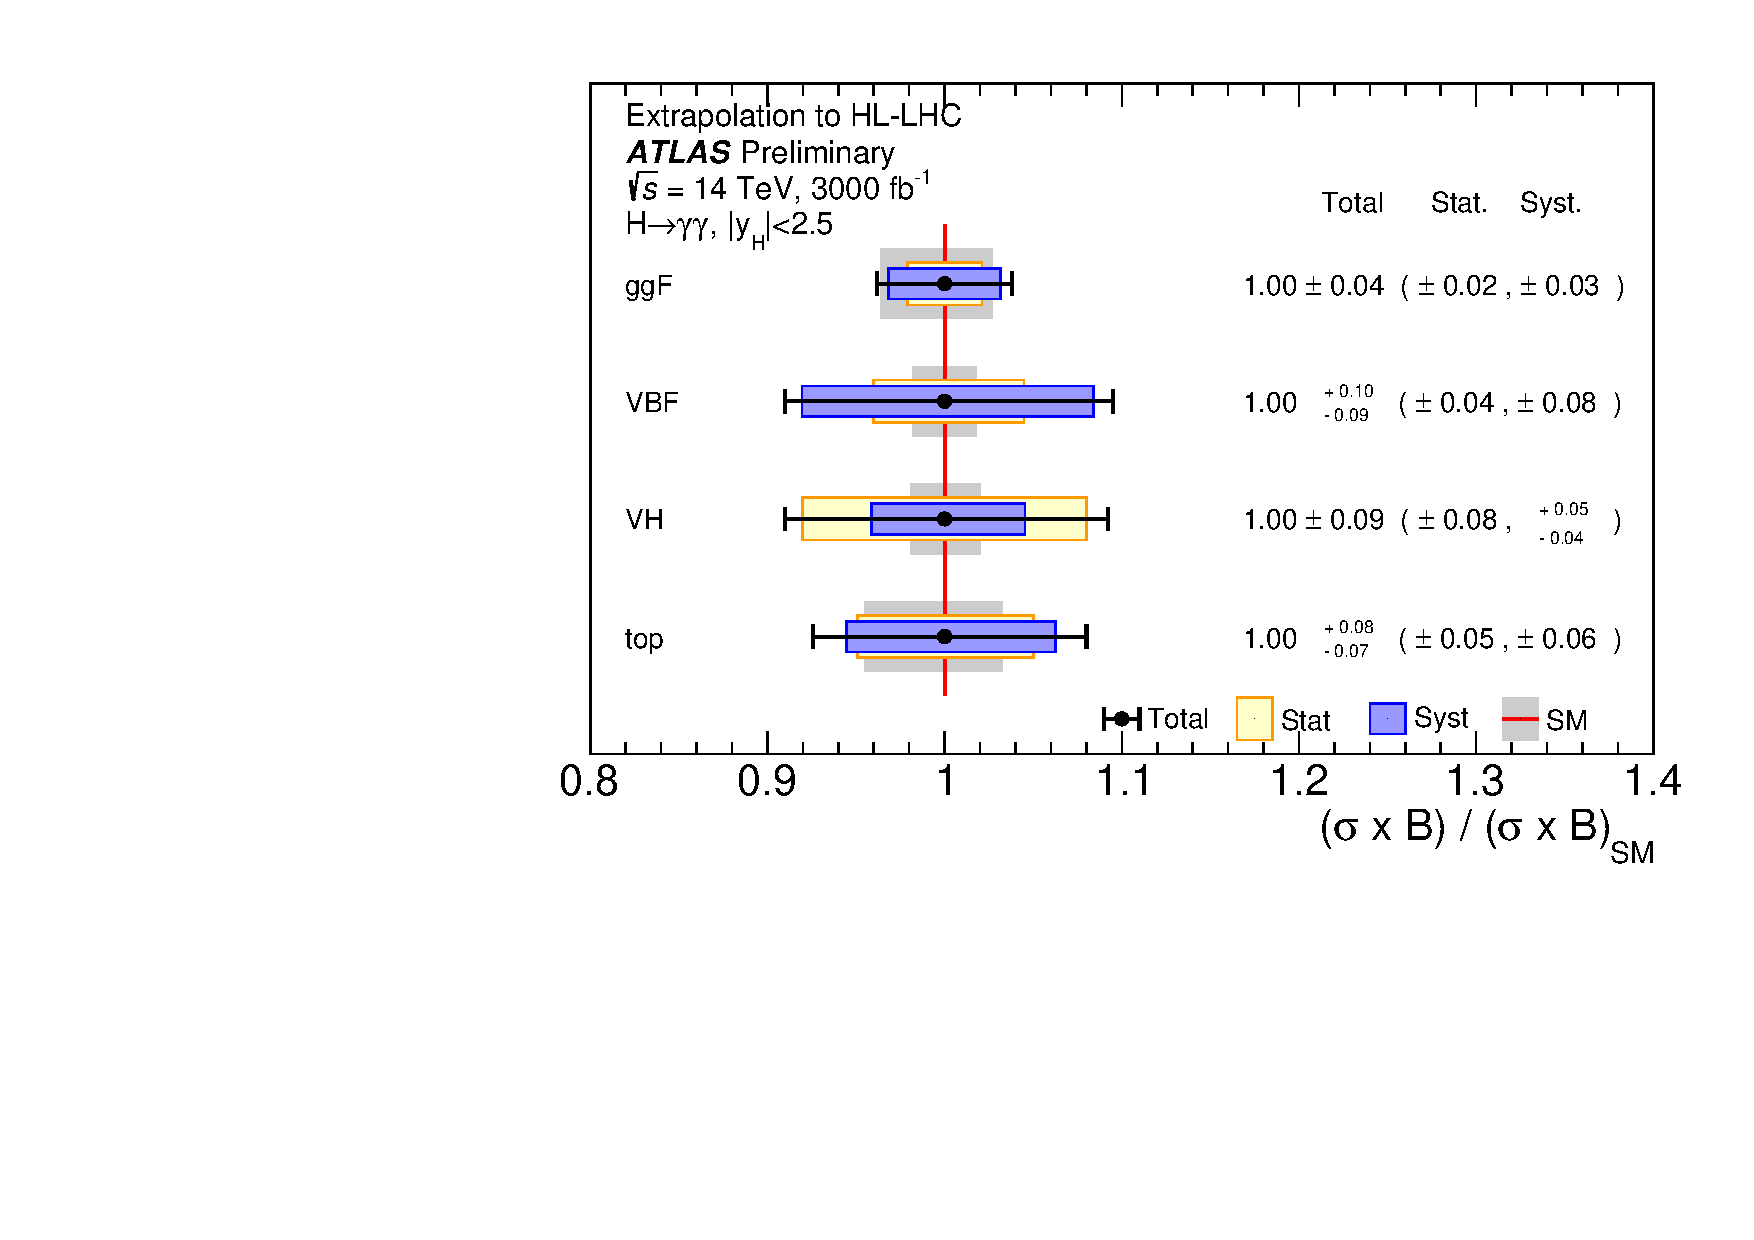
\includegraphics[width=0.56\linewidth]{\main/section2/plots/channels/ATLAS_plot_compareToSM_yy_prodXS}
  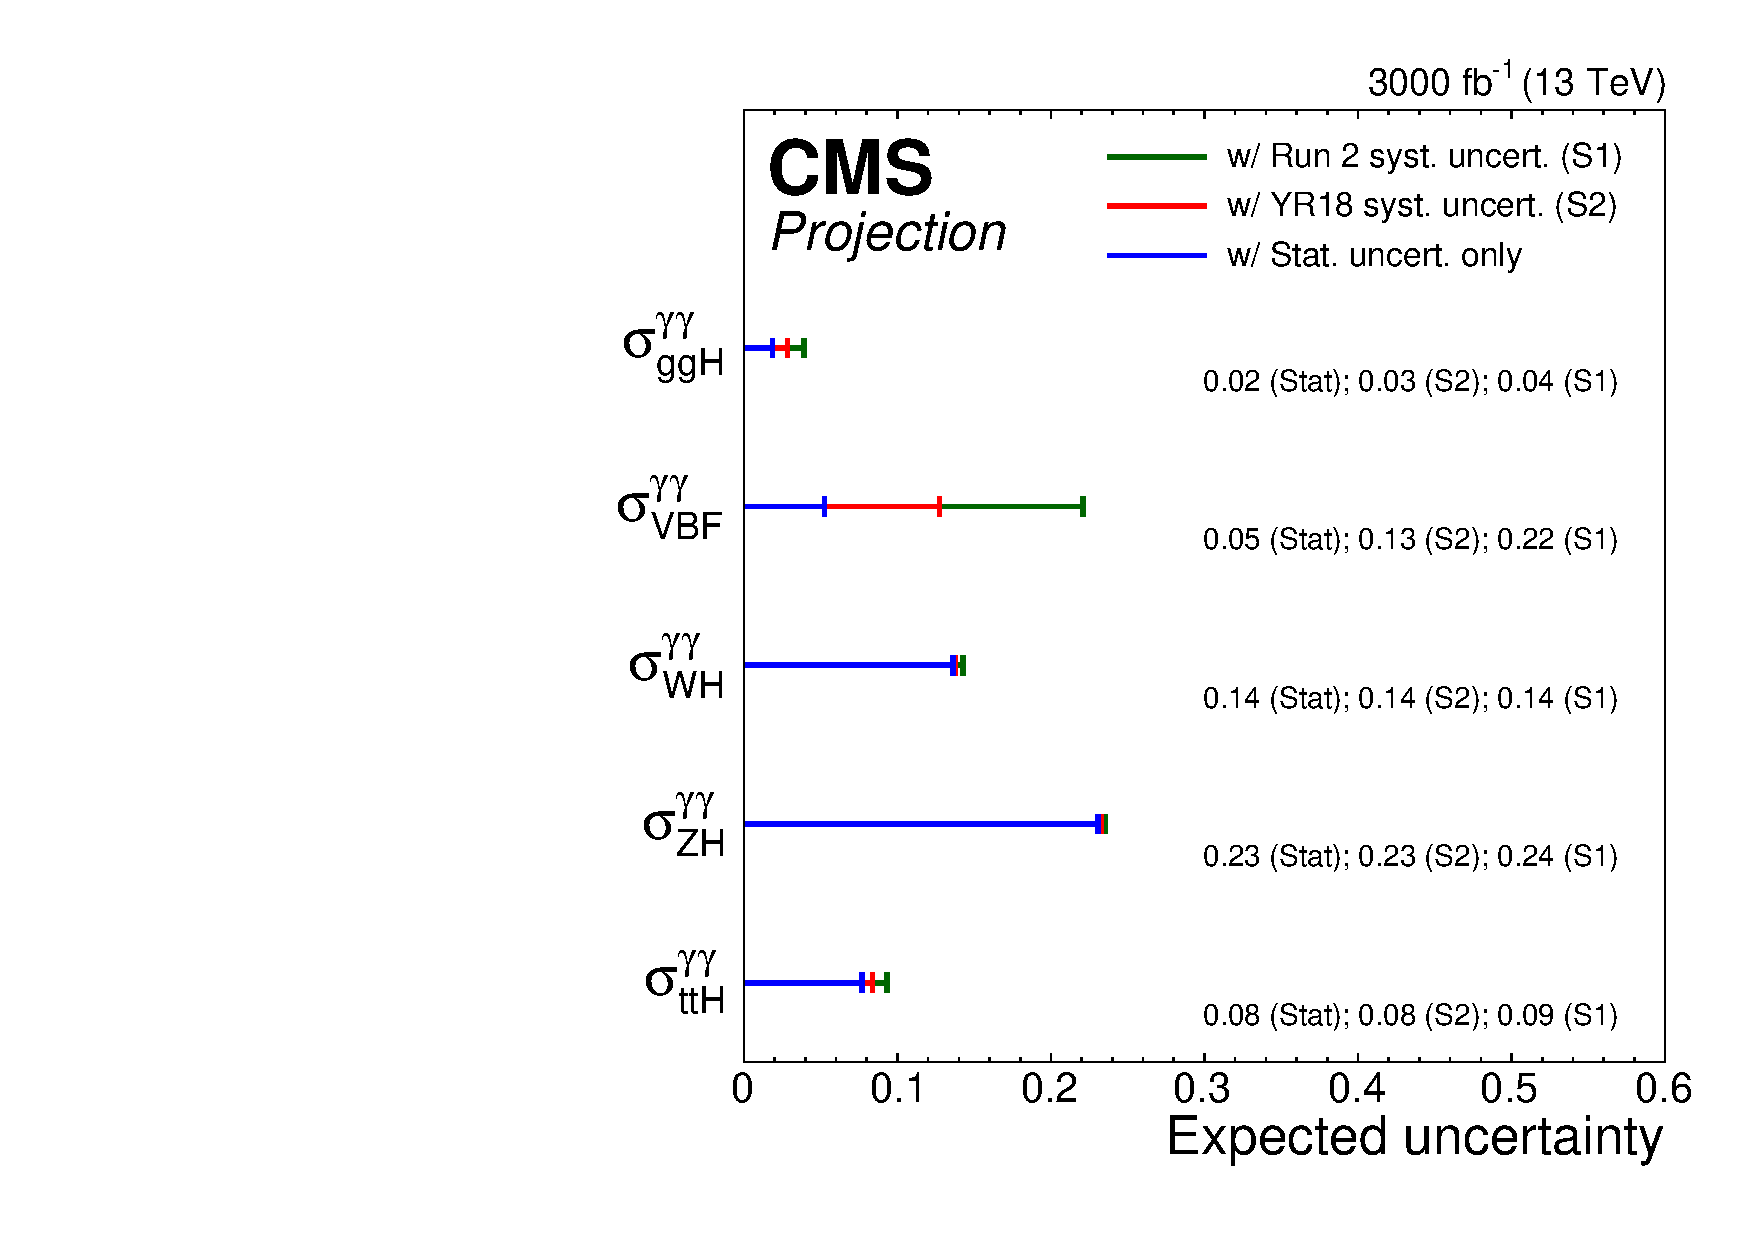
\includegraphics[width=0.42\linewidth]{\main/section2/plots/channels/CMS_summary_A1_5PD_3000_hgg}
  \caption{Cross-section times branching fraction measurements of the main Higgs production modes in the \Hyy\ decay channel, as extrapolated at the HL-LHC. In case of ATLAS results (left) the ratios of cross sections to their respective theoretical SM predictions are shown for scenario S2, while in case of CMS results (right) the uncertainties on these measurements are shown for S1, S2, and Stat-only scenarios..}
  \label{fig:Hyy_ATLAS_HLLHC_S2}
\end{figure}

\subsubsection{$H \to Z\gamma \to \ell\ell\,\gamma$}
%%{\it To be written by: M. Delmastro}

Due to the small branching fraction in the SM, the \HZy\ decay has not yet been observed at the LHC. The experimental observed limits at the $95\%$ confidence level are currently 6.6 times the SM prediction for a Higgs boson mass of 125.09 GeV by ATLAS and 3.9 times the SM prediction for a Higgs boson mass of 125 GeV by CMS, based on the analyses of 36\,$\mathrm{fb}^{-1}$ of $pp$ collision at $\sqrt{s} = 13$ TeV described in Ref. \cite{Aaboud:2017uhw, Sirunyan:2018tbk}.

The analyses select events with an isolated photon candidate passing good quality requirements in the precision regions of the detectors, and a dilepton system with properties compatible with that of the decay of a $Z$ boson. Events are separated according to lepton flavour, the event kinematic properties, and the presence of jets compatible with the VBF production of the Higgs boson, in order to maximize the signal sensitivity. The signal is sought for by means of a combined signal-plus-background fit of the photon-dilepton invariant mass spectra in various event categories, where both the continuous background and the signal resonance are parameterized by analytical functions. The Run-2 analyses are strongly driven by statistical uncertainty, and the main systematic uncertainties are from the bias associated to the background modeling.

The extrapolations to HL-LHC are performed with a simple scaling approach, assuming the same signal and background modeling used in the Run-2 analyses. All experimental and systematic uncertainties are considered to remain the same (S1), except the uncertainty associated to the background modeling, which is taken to be negligible.

The ATLAS expected significance to the SM Higgs boson decaying in $Z\gamma$ is 4.9 $\sigma$ with 3000\,$\mathrm{fb}^{-1}$. Assuming the SM Higgs production cross section and decay branching ratios, the signal strength is expected to be measured with a $\pm0.24$ uncertainty. The cross section times branching ratio for the $pp\rightarrow H \rightarrow Z\gamma$ process is projected to be measured as $1.00\pm0.23$ times the SM prediction. Even at the HL-LHC scenario S1, the analysis sensitivity  to \HZy\ will remain driven by the statistical uncertainty. The dominant source of systematic uncertainty in the extrapolation is that associated to the 
%% QCD scale variations.
missing higher order uncertainties.

\subsubsection{$H \to ZZ^* \to 4\ell$}
%% {\it To be written by: M. Delmastro}

The measurement of the Higgs boson properties in the \HZZ\ channel is performed using the events that contain at least two same-flavour opposite-sign dilepton pairs, chosen from isolated electrons and muons candidates passing good quality requirements in the precision regions of the detectors. Additional constraints on the kinematical properties of the lepton pair associated with the decay of the on-shell $Z$ boson, and on the global topology of the event, helps to improve the signal to background ratio. The four-lepton invariant mass resolution is improved by correcting for the emission of final-state radiation photons by the leptons.
%%
The \HZZ\ signal is extracted from the four-lepton invariant mass spectra in the different event categories, after having evaluated the background components using simulations to constrain their shapes, and data control regions to extrapolate their normalization in the signal regions. Signal to background sensitivity is in general enhanced using the multivariate and/or matrix-element based techniques. More details on the analyses methods can be found in most recent measurements in the \HZZ\ channel published by ATLAS \cite{ATLAS:2018bsg} and CMS \cite{Sirunyan:2017exp}.

The performance of the measurement of the Higgs boson properties in the \HZZ\ at HL-LHC is extrapolated from the most recent measurements by ATLAS with 80\,$\mathrm{fb}^{-1}$ \cite{ATLAS:2018bsg}, and by CMS with 36\,$\mathrm{fb}^{-1}$ \cite{Sirunyan:2017exp}. The dominant systematic uncertainties affecting the extrapolation of the ggH cross section measurement are the lepton reconstruction and identification efficiencies, and pile-up modeling uncertainties. The VBF and VH cross-sections are primarily affected by the uncertainty on the jet energy scale and resolution, and by the
%% QCD scale uncertainties.
missing higher order uncertainties.
These and
%% The theory uncertainties related to QCD scale
the parton shower modeling primarily affects the extrapolated top cross section.

The VBF, VH and especially top measurements in the \HZZ\ decay channel remain largely dominated by statistical uncertainty when extrapolated to 3000\,$\mathrm{fb}^{-1}$ while the $ggH+b\bar{b}H$ cross section is dominated by systematic uncertainties both in scenario S1 and S2.
%
Figure~\ref{fig:HZZ_ATLAS_HLLHC_S2} shows the ratio of the extrapolated \HZZ\ ATLAS measurements of the main Higgs boson production modes to their respective theoretical SM predictions in the scenario S2 (left), and uncertainties on these measurements for S1, S2, and stat-only scenarios as extrapolated using the \HZZ\ CMS measurements (right). The ggF and top \HZZ\ measurements at HL-LHC are expected to reach a level of precision comparable to the projected uncertainty on the corresponding theory predictions.

\begin{figure}
  \centering
  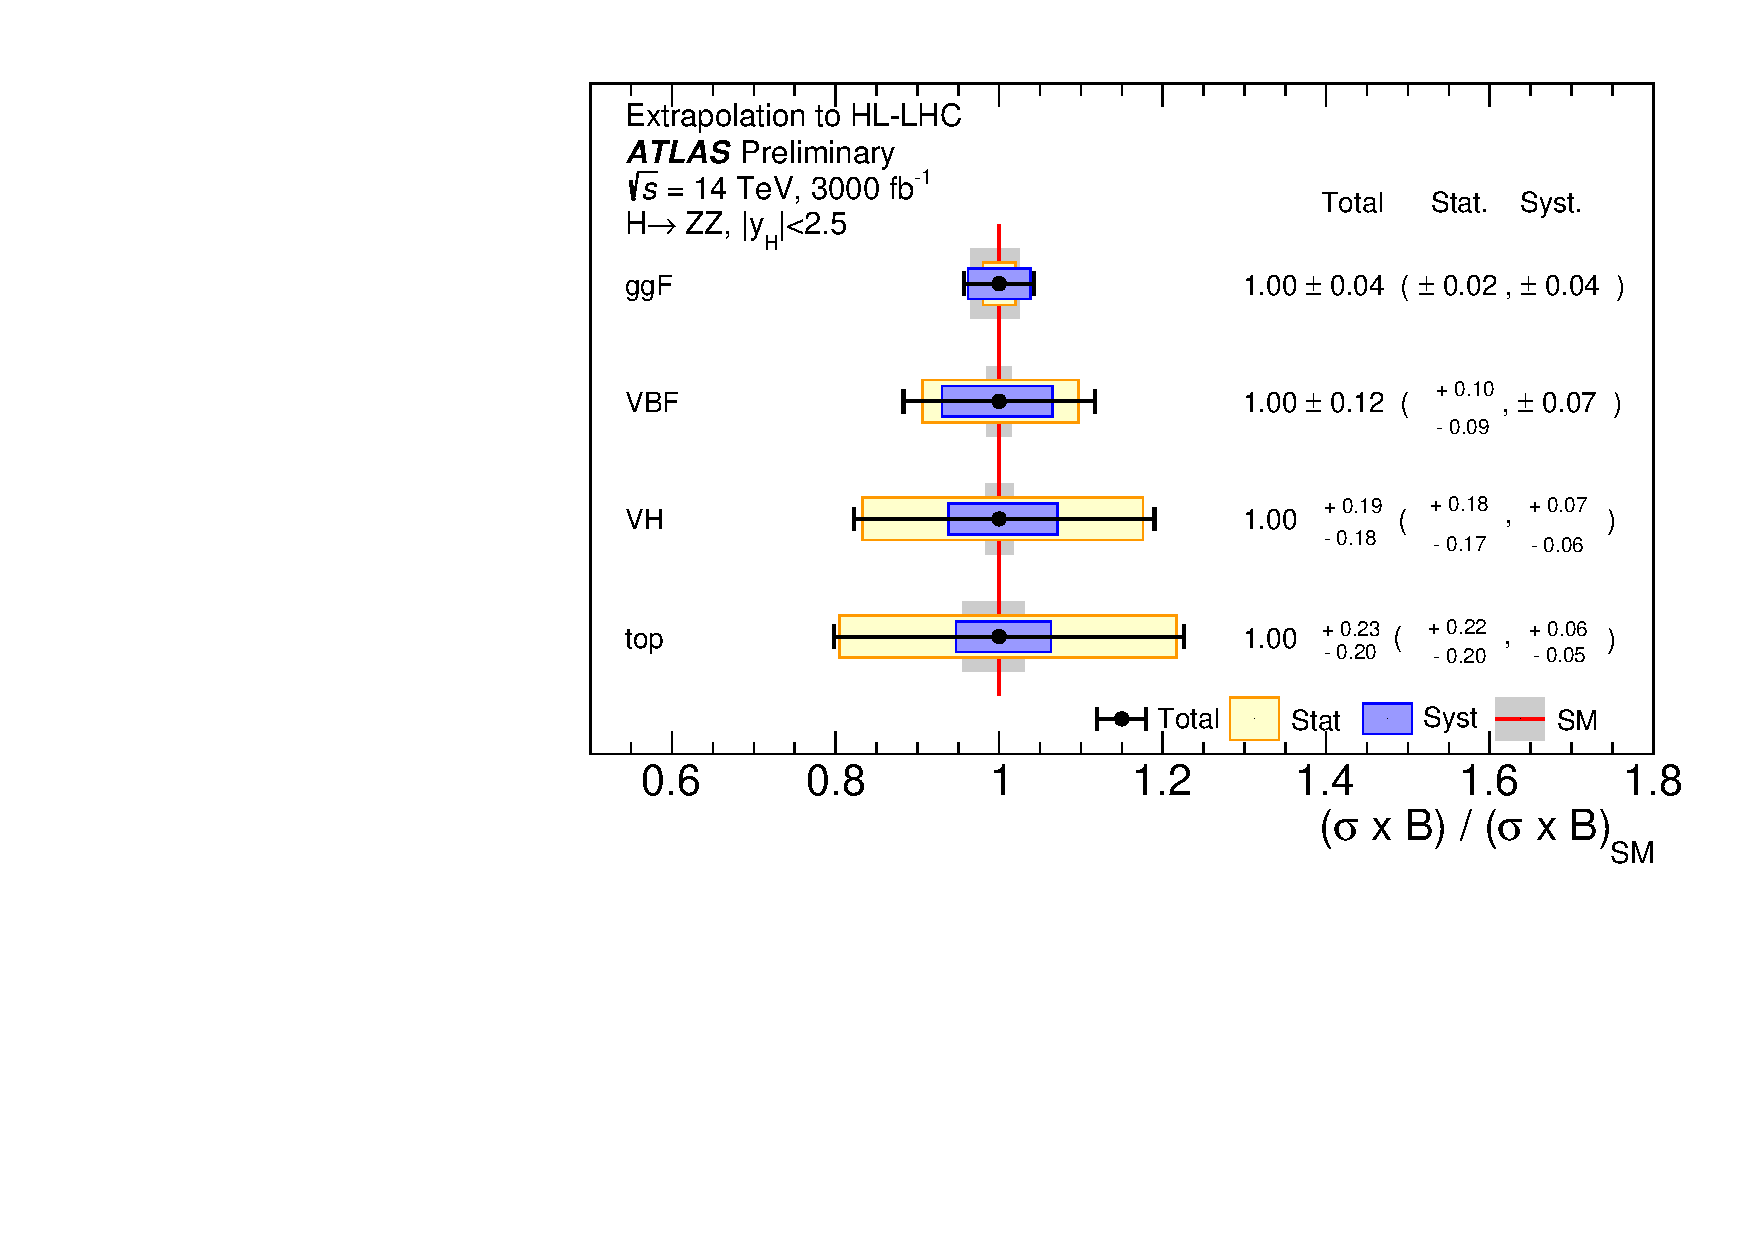
\includegraphics[width=0.56\linewidth]{\main/section2/plots/channels/ATLAS_plot_compareToSM_ZZ_prodXS}
  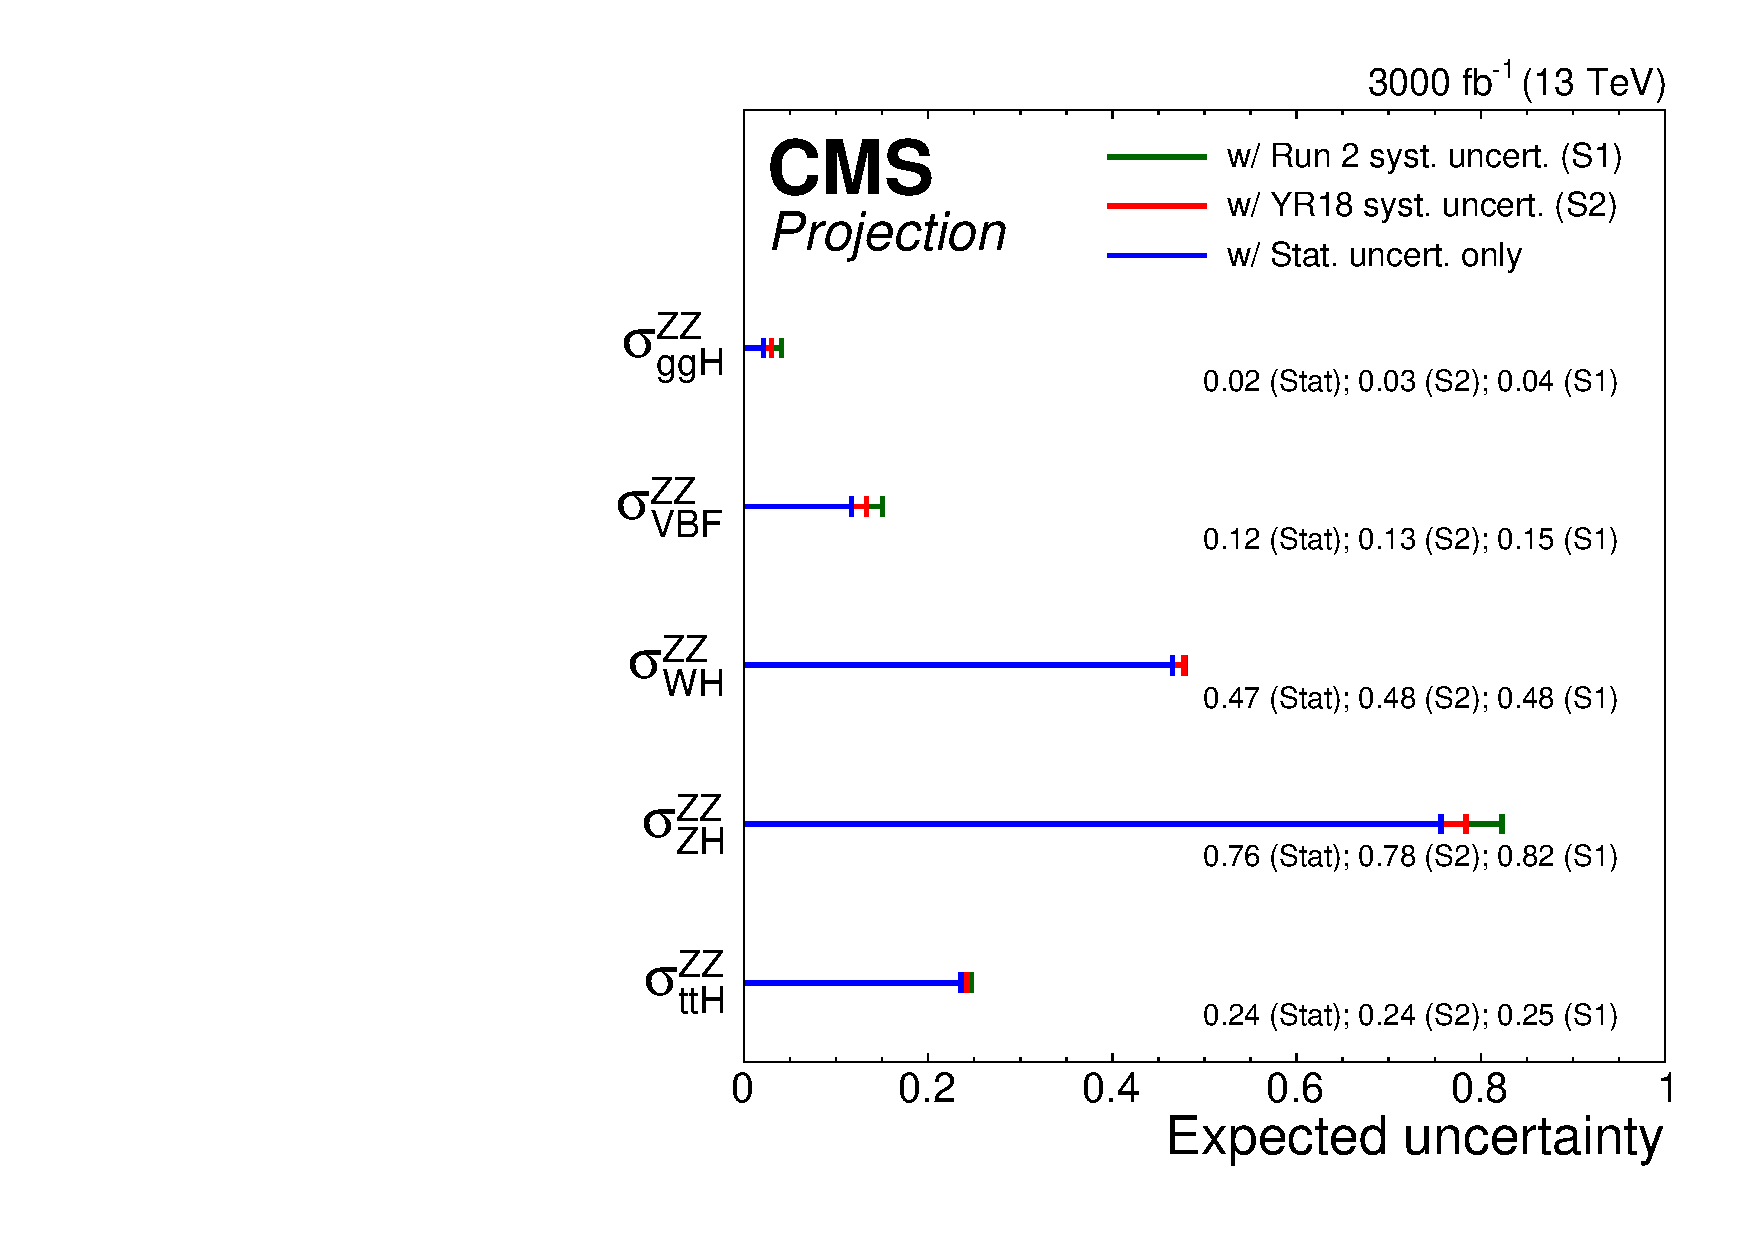
\includegraphics[width=0.42\linewidth]{\main/section2/plots/channels/CMS_summary_A1_5PD_3000_hzz}
  \caption{Cross-section times branching fraction measurements of the main Higgs boson production modes in the \HZZ\ decay channel, as extrapolated at the HL-LHC. In case of ATLAS results (left) the ratios of cross sections to their respective theoretical SM predictions are shown for scenario S2, while in case of CMS results (right) the uncertainties on these measurements are shown for S1, S2, and Stat-only scenarios.}
  \label{fig:HZZ_ATLAS_HLLHC_S2}
\end{figure}

\subsubsection{$H \to WW^* \to \ell\nu\,\ell\nu$}
%% {\it To be written by: M. Delmastro}

The measurement of the Higgs boson properties in the \HWW\ channel is performed using the events that contain two opposite-charged isolated leptons passing good quality requirements in the precision region of the detectors and missing transverse momentum. Additional requirements on the event kinematical properties are applied to reduce the various background components (e.g. requirements on the dilepton invariant mass, transverse mass of the di-lepton + MET system). Events are categorized as a function of the jet multiplicity in order to exploit the different background composition in different categories, and to help extracting the Higgs ggH and VBF production cross sections. The normalizations of the top ($t\bar{t}$ and $W+t$), and $Z\rightarrow\tau\tau$ backgrounds are set using dedicated control regions of the same jet multiplicity as the signal category to which the normalization is transferred. In case of the (non-resonant) $WW$ background, its normalization is either determined using dedicated control regions (ATLAS approach) or by using theoretical prediction with corresponding uncertainty on it (CMS approach). More details on the analyses methods can be found in most recent measurements in the \HWW\ channel published by ATLAS \cite{Aaboud:2018jqu} and CMS \cite{Sirunyan:2018egh}.

The performance of the measurements of Higgs boson properties in the \HWW\ channel at HL-LHC is extrapolated from the most recent measurements in this channel performed by ATLAS with 80\,$\mathrm{fb}^{-1}$ \cite{Aaboud:2018jqu} and by CMS with 36\,$\mathrm{fb}^{-1}$ \cite{Sirunyan:2018egh}. These measurements are completely dominated by systematic uncertainties, and their extrapolation to the S2 scenario shows the expected reduction by a factor two. The measurement of the ggH cross section by branching fraction is dominated by theoretical PDF uncertainty, followed by experimental uncertainties affecting the signal acceptance, including uncertainties on the jet energy scale and flavour composition, and lepton misidentification; the VBF result suffers from similar dominant uncertainties.
%%
Figure~\ref{fig:HWW_ATLAS_HLLHC_S2} shows the ratio of the extrapolated \HWW\ ATLAS measurements of the main Higgs production modes to their respective theoretical SM predictions in scenario S2 (left), and uncertainties on these measurements for S1, S2, and Stat-only scenarios as extrapolated using the \HWW\ CMS measurements (right).

\begin{figure}
  \centering
  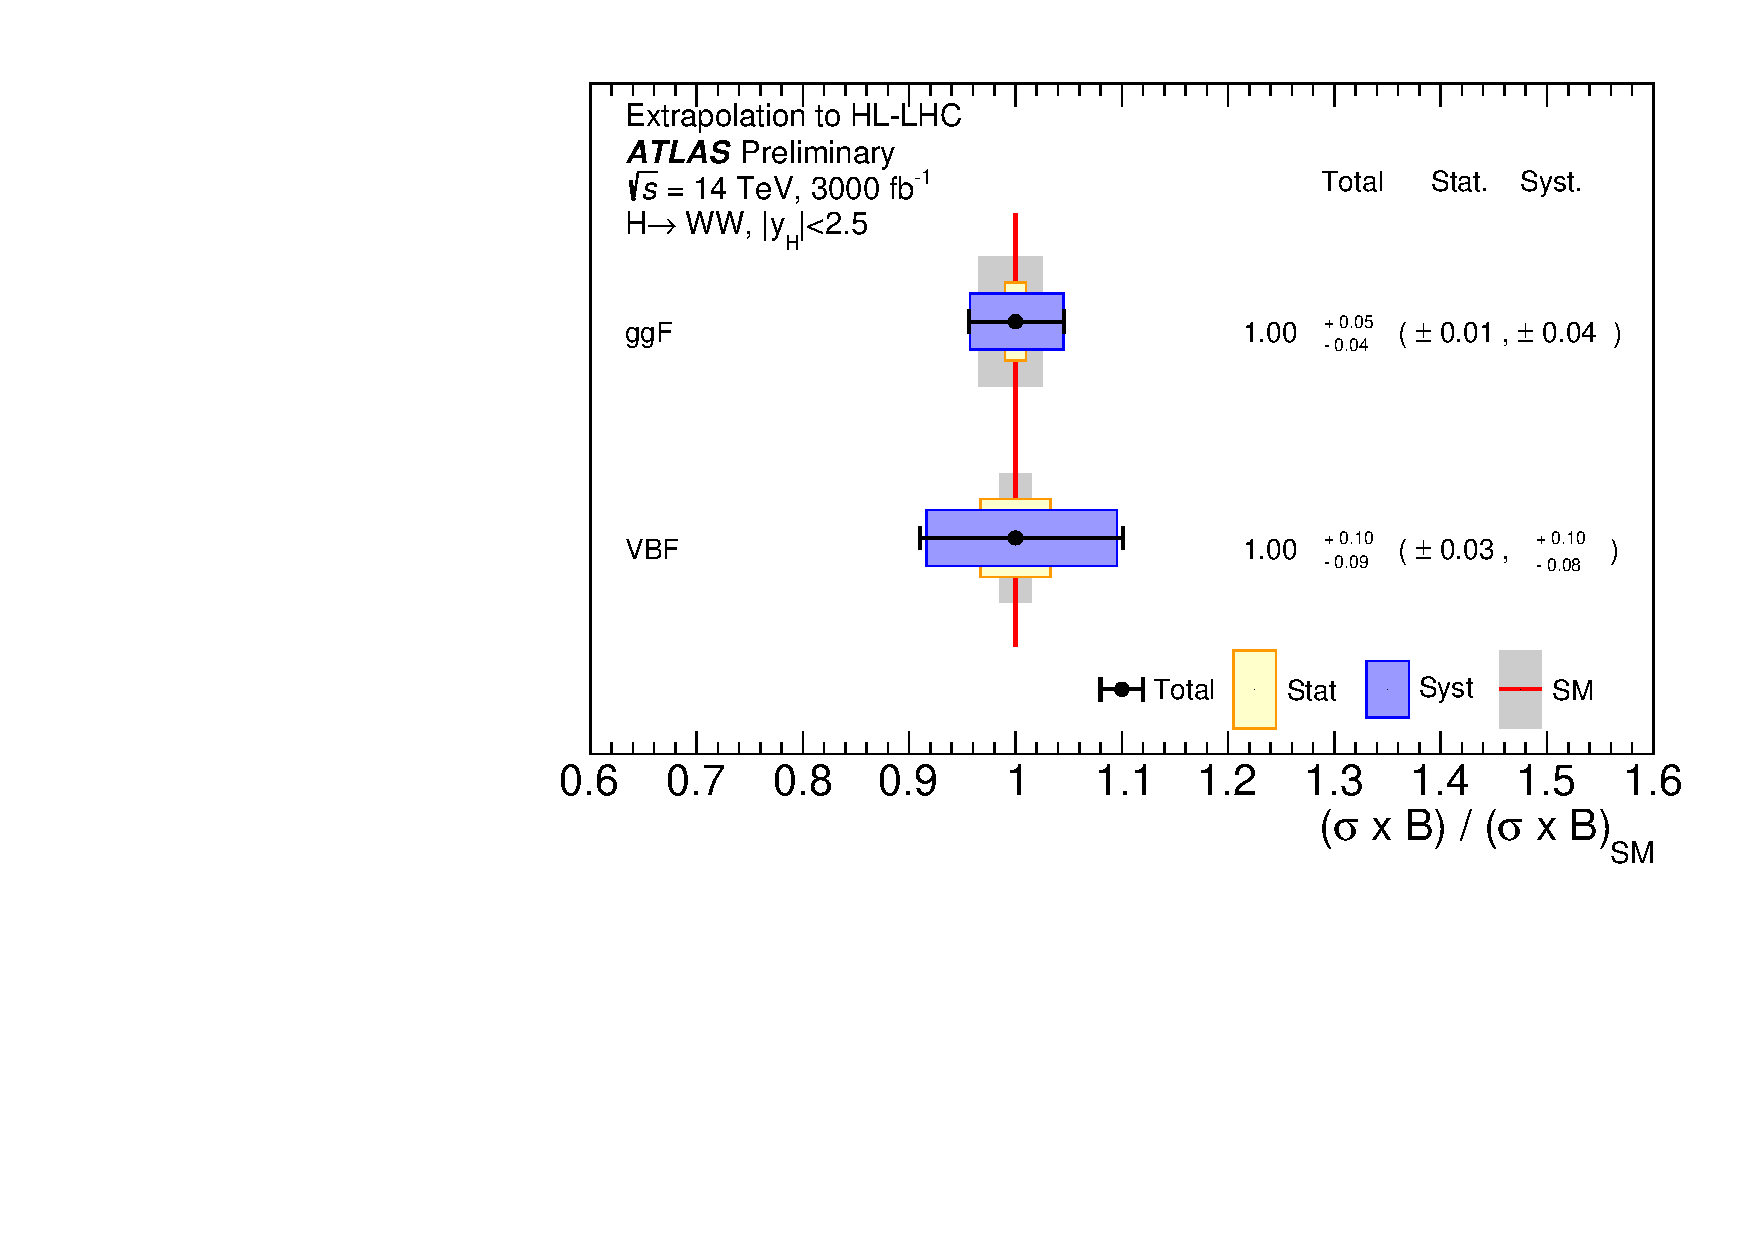
\includegraphics[width=0.56\linewidth]{\main/section2/plots/channels/ATLAS_plot_compareToSM_WW_prodXS}
  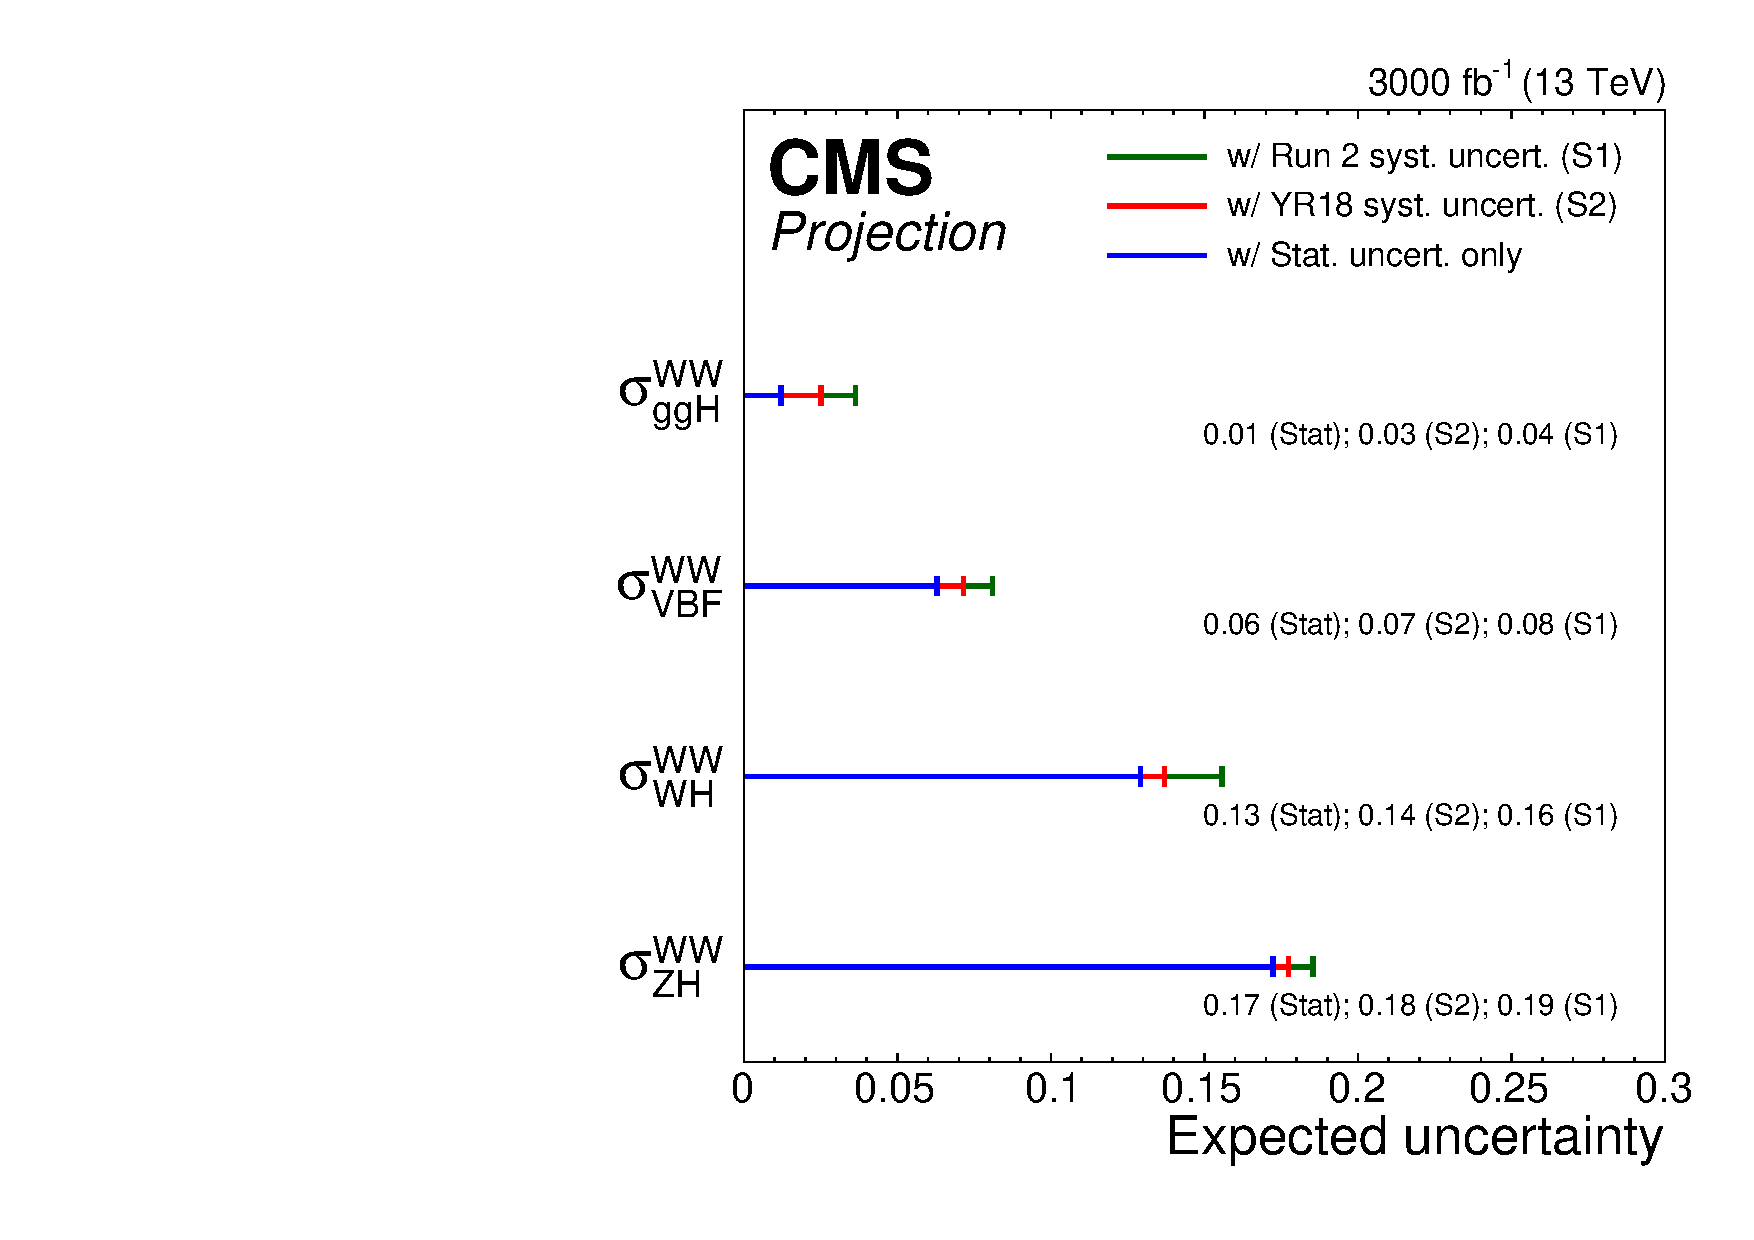
\includegraphics[width=0.42\linewidth]{\main/section2/plots/channels/CMS_summary_A1_5PD_3000_hww}
  \caption{Cross-section times branching fraction measurements of the main Higgs production modes in the \HWW\ decay channel, as extrapolated at the HL-LHC. In case of ATLAS results (left) the ratios of cross sections to their respective theoretical SM predictions are shown for scenario S2, while in case of CMS results (right) the uncertainties on these measurements are shown for S1, S2, and Stat-only scenarios.}
  \label{fig:HWW_ATLAS_HLLHC_S2}
\end{figure}


\subsubsection{$H \to \tau^{+}\tau^{-}$}
%\begin{center}
%  \textit{Written by: P. Francavilla}
%\end{center}
The measurement of the Higgs boson  in the $H \to \tau^{+}\tau^{-}$ channel considers the leptonic ($\tau_{lep}$) and the hadronic ($\tau_{had}$) decays of the $\tau$ lepton. Three subs-channels ($\tau_{lep}\tau_{lep}$, $\tau_{lep}\tau_{had}$ and $\tau_{had}\tau_{had}$) are defined by requirements on the number of hadronically decaying $\tau$-leptons candidates and leptons (electrons or muons) in the event.
Candidate events are divided into categories using kinematic properties to target cases in which the Higgs boson is produced with a  boost ($\pT > 100$ GeV), primarily from gluon  fusion, and cases primarily produced from vector boson fusion, in which the Higgs boson is produced with two jets separated in pseudo-rapidity. Additional requirements are employed to discriminate signal from background. One of the most important variable is the mass of the $\tau\tau$ system, calculated in ATLAS with the Missing Mass Calculator \cite{Elagin:2010aw}.
The normalization of the dominant backgrounds ($Z\to\ell^{+}\ell^{-}$, $t\bar{t}$, Fake-$\tau_{had}$) is determined using dedicated control regions, or extracted directly in each signal region ($Z\to\tau^{+}\tau^{-}$, the dominant and irreducible background).  More details on the analysis methods can be found in the most recent measurements in the  $H \to \tau^{+}\tau^{-}$ channels published by ATLAS \cite{ATLAS-CONF-2018-021} and CMS \cite{Sirunyan:2017khh}.

%dataset of the extrapolation
The studies presented here are performed based on a previous analysis, in which the ATLAS Collaboration analyzed the 2015/2016 proton-proton collision dataset collected at $\sqrt{s} = 13\,\UTeV$, which corresponds to an integrated luminosity of 36.1\fbinv \cite{ATLAS-CONF-2018-021}. 
%results
The measurements of the cross sections for the gluon fusion and vector boson fusion production modes are dominated by systematic uncertainties, as can be seen in  Table \ref{tab:htt_proj}, which  lists the total expected uncertainties on the cross sections normalised to their SM values as well as  the different contributions from different types of uncertainties. 
The dominant contributions, the experimental and background modelling errors, are due to uncertainties on jet calibration and resolution, on the reconstruction of the $E_{T}^{miss}$, and on the determination of the background normalization from signal and control regions.
These results are compared to the SM prediction in Figure \ref{fig:htt_proj}; the SM uncertainties are divided by two compared to their current values, which approximately corresponds to the scaling expected from S2  scenario. The figure shows that at the HL-LHC the measurement will reach a level of precision which is  similar to the theory predictions. These systematic uncertainties are dominated by the theoretical errors on the signal acceptance for the gluon fusion measurement both for S1 and S2. In the measurement of the vector boson fusion cross section, the effects of the experimental errors and uncertainties on the background modelling become more relevant, expecially in S2. 
\begin{table}[th!]
\begin{center}
{
\caption{Expected results for the production mode cross-section measurement in the $H\to \tau^{+} \tau^{-}$ channel with 36\fbinv of Run 2 data and at the HL-LHC. Uncertainties are reported relative to the SM cross section at the corresponding center-of-mass energy. Both scenarios have been considered for the systematic uncertainties in the HL-LHC extrapolation.}
\label{tab:htt_proj}
\begin{tabular}{l | c c c c}
\hline\hline\\
Experiment, Process & \multicolumn{2}{c}{ATLAS, ggF}& \multicolumn{2}{c}{ATLAS, VBF}\\ 
\hline\\
Scenario &  S1 & S2 & S1 & S2  \\
%Luminosity & 79.8 \fbinv&\multicolumn{2}{c}{3000 \fbinv}& 79.8 \fbinv&\multicolumn{2}{c}{3000 \fbinv}\\
Total uncertainty   & xx\%& xx\%  & xx\% & xx\%\\
\hline
Statistical uncert.  & xx\%& xx\%  & xx\% & xx\%\\
Experimental uncert. & xx\%& xx\%  & xx\% & xx\%\\
Signal theory uncer. & xx\%& xx\%  & xx\% & xx\%\\
Background theory uncer. & xx\%& xx\%  & xx\% & xx\%\\
\hline\hline
\end{tabular}
} % end footnotesize
\end{center}
\end{table}
 \begin{figure}[h!]
\begin{center}
%%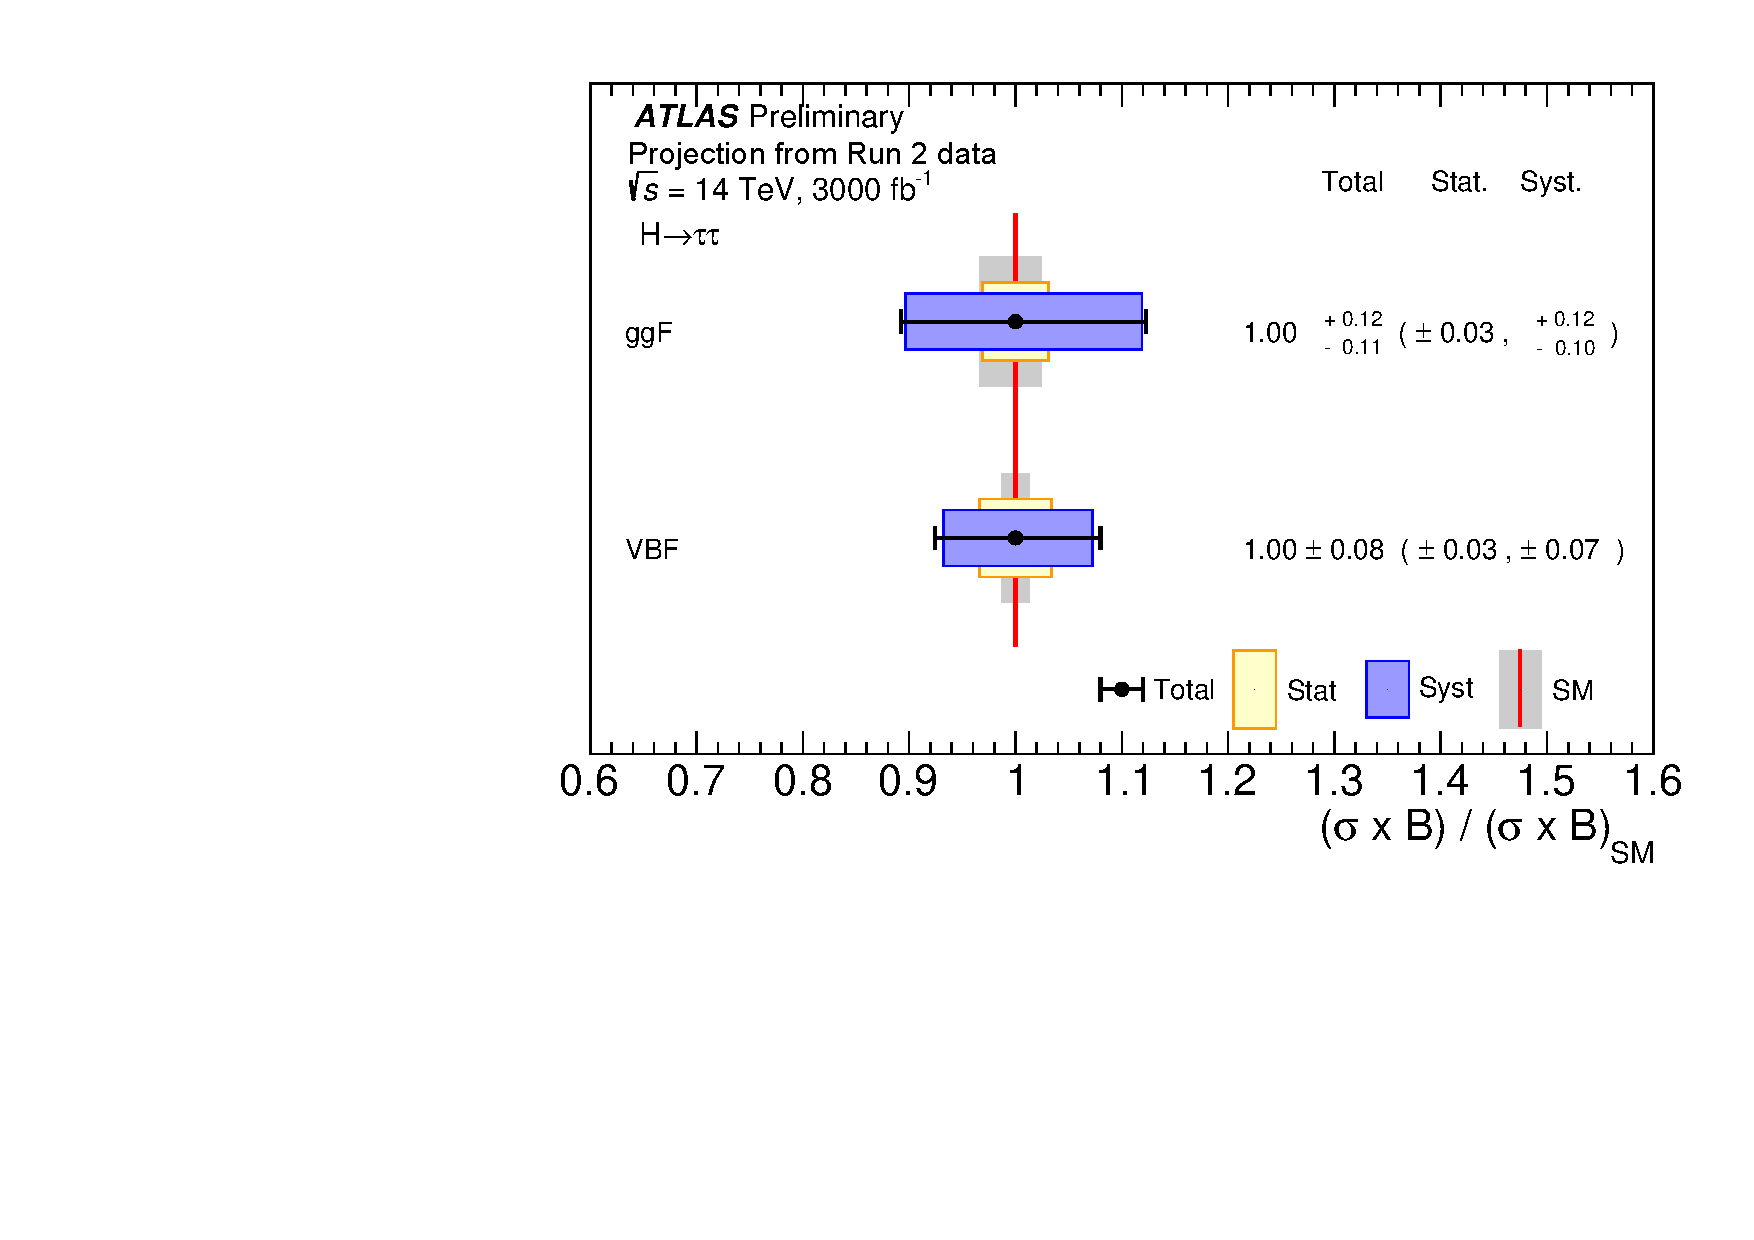
\includegraphics[width=0.6\textwidth]{htauATLAS.png}
\end{center}
\caption{Comparison, for $H \to \tau^{+}\tau^{+}$ final state applying scenario S2, between the expected precision on production-mode cross section times branching ratio normalised to their SM expectation at HL-LHC and the theoretical uncertainty on the SM prediction. 
}
\label{fig:htt_proj}
\end{figure}


\subsubsection{$H \to b\bar{b}$}
%\begin{center}
%{\it Written by: P. Francavilla, A. de Wit}
%\end{center}
%\wip{Text currently reflects CMS studies only. Should be updated to reflect ATLAS and CMS studies.
%Differences for ATLAS: 
%-> the analysis is the observation (78.9 fb-1)
%-> tagger is named MVa, and we use a 70\% WP
%-> mbb is improved with muon in jet correction and ptReco, + kinematic fit for 2 leptons
%-> add the mu for ATLAS
%-> Add the results from ATLAS
%}

%dataset of the extrapolation
The measurement of the Higgs boson  in the $H \to b\bar{b}$ channel presented here considers the Higgs boson production in assoculation with a vector boson ($V=W/Z$). 
Searches for the  $H \to b\bar{b}$  in association with a vector boson drove the recent observation  of this decay mode reported by the ATLAS and CMS Collaborations \cite{Aaboud:2018zhk,Sirunyan:2018kst}.
The analyses make use of leptonic decays of the vector boson for triggering and to reduce the multi-jet background: the final states
of the $\vh$ system covered in the analyses always contain two b-jets and either zero, one or two electrons or muons. Both leptons are required to have the same flavour in the two lepton selection.
%backgrounds
Major backgrounds arising from SM production of vector boson plus heavy- or light-flavour jets, in addition to $t\bar{t}$ production, are 
controlled and constrained via dedicated control regions. The  b-jet energy resolution is improved by using multivariate energy regression techniques (CMS), or sequential corrections (ATLAS), and a boosted decision tree is used to improve the discrimination 
between signal and background. The distribution of this multivariate discriminator is used as the discriminating
variable in the signal extraction fit. 

The ATLAS and CMS Collaborations have both recently reported the observation of the $H \to b\bar{b}$ decay \cite{Aaboud:2018zhk,Sirunyan:2018kst}.
The studies presented here are performed by extrapolating this most recent ATLAS $H \to b\bar{b}$ measurements using a dataset corresponding to an integrated luminosity of 78.9 \fbinv, and by extrapolating a previous analysis by the CMS Collaboration. In this previous analysis evidence for the$H \to b\bar{b}$ decay in the $\text{VH}$ production mode was reported using a dataset corresponding to an integrated luminosity of 35.9\fbinv \cite{HIG16044}. 

%channels

%results
%The signal strength observed in the CMS analysis is 
%$\mu_{\text{VHbb}} = 1.19^{+0.21}_{-0.20}\text{ (stat) }^{+0.34}_{-0.32}\text{ (syst) }$. The projected uncertainties on the signal strength reported here %assume $\mu_{\text{vHbb}} = 1$.

Figure \ref{fig:vhbb_proj_bars} shows the extrapolation of the signal strength uncertainty per-channel (CMS) and per-production mode (ATLAS). The details of the contributions of different sources of uncertainty in scenarios S1 and S2 for the projection of the ATLAS and CMS analyses are shown in Table~\ref{tab:vhbb_uncertbreakdown}.
%These results are for the projection of the CMS analysis.
The large improvement, by a factor 2.5--3, in the uncertainty of the measurement for the $WH$ (1-lepton channel) compared to the Run-2 results (around 45\%) is caused by the integrated luminosity scaling of the uncertainty in the modelling of the $W$ boson $\pT$ distribution for both the collaborations, being the dominant uncertainty in scenario S1.

\begin{figure}[h!]
\begin{center}
% 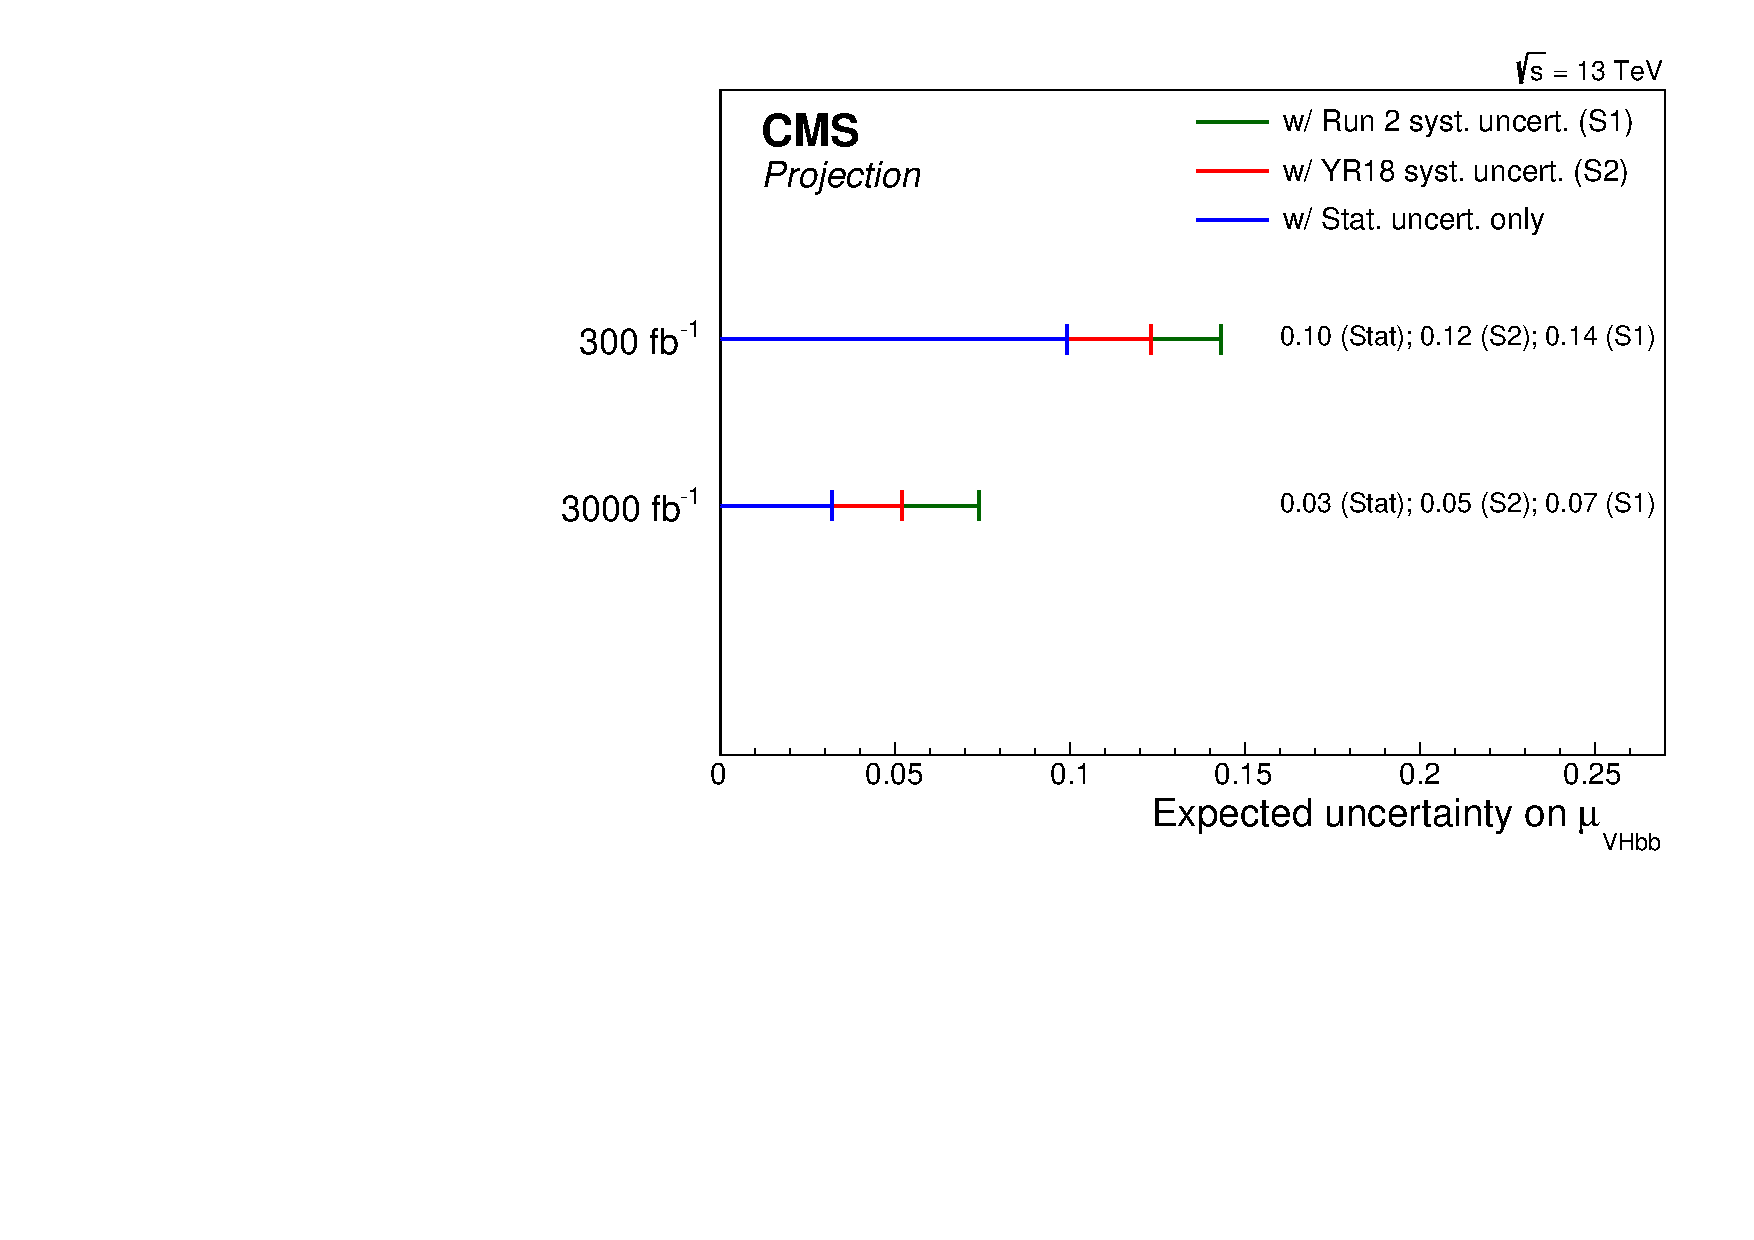
\includegraphics[width=0.48\textwidth]{\main/section2/plots/channels/Uncert300and3000.pdf}
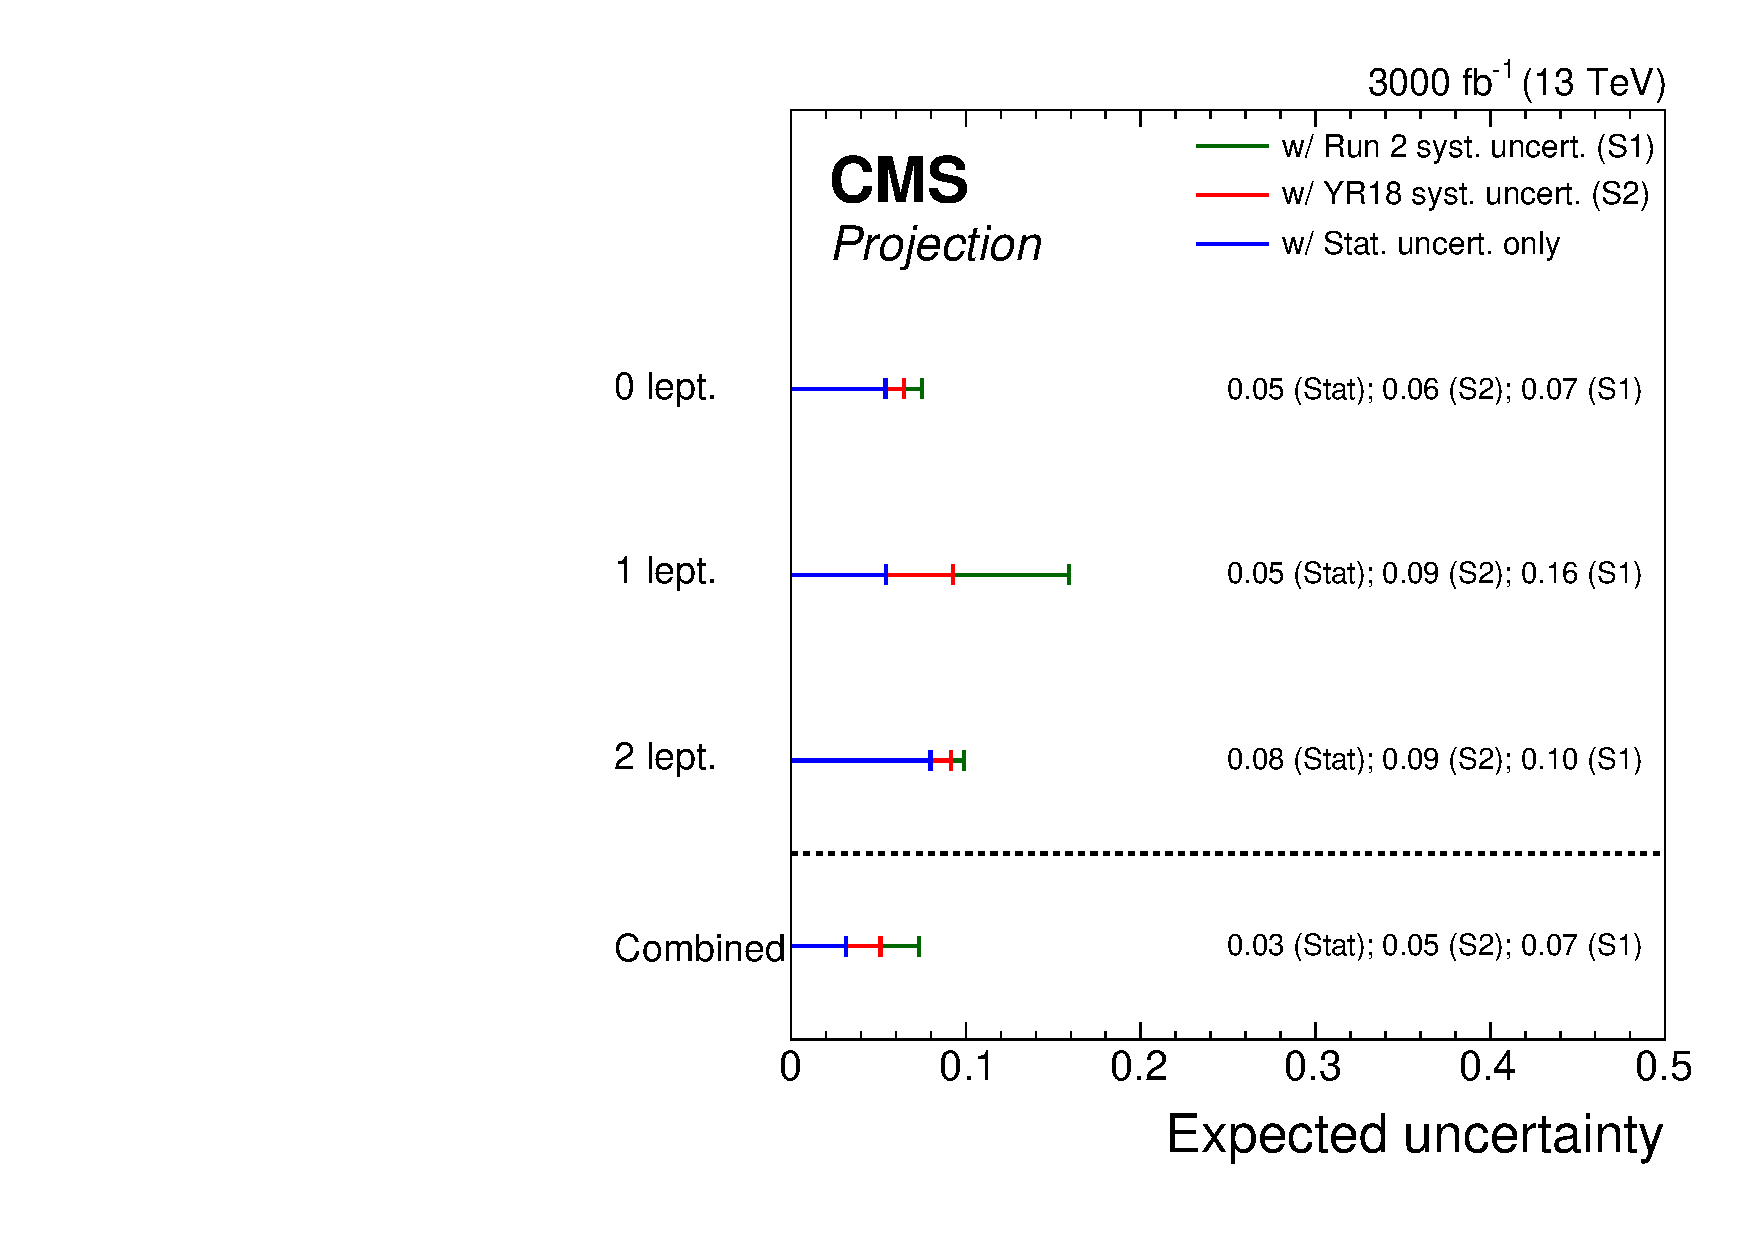
\includegraphics[width=0.45\textwidth]{\main/section2/plots/channels/ccc_3000fb_all_condensed.pdf}
%%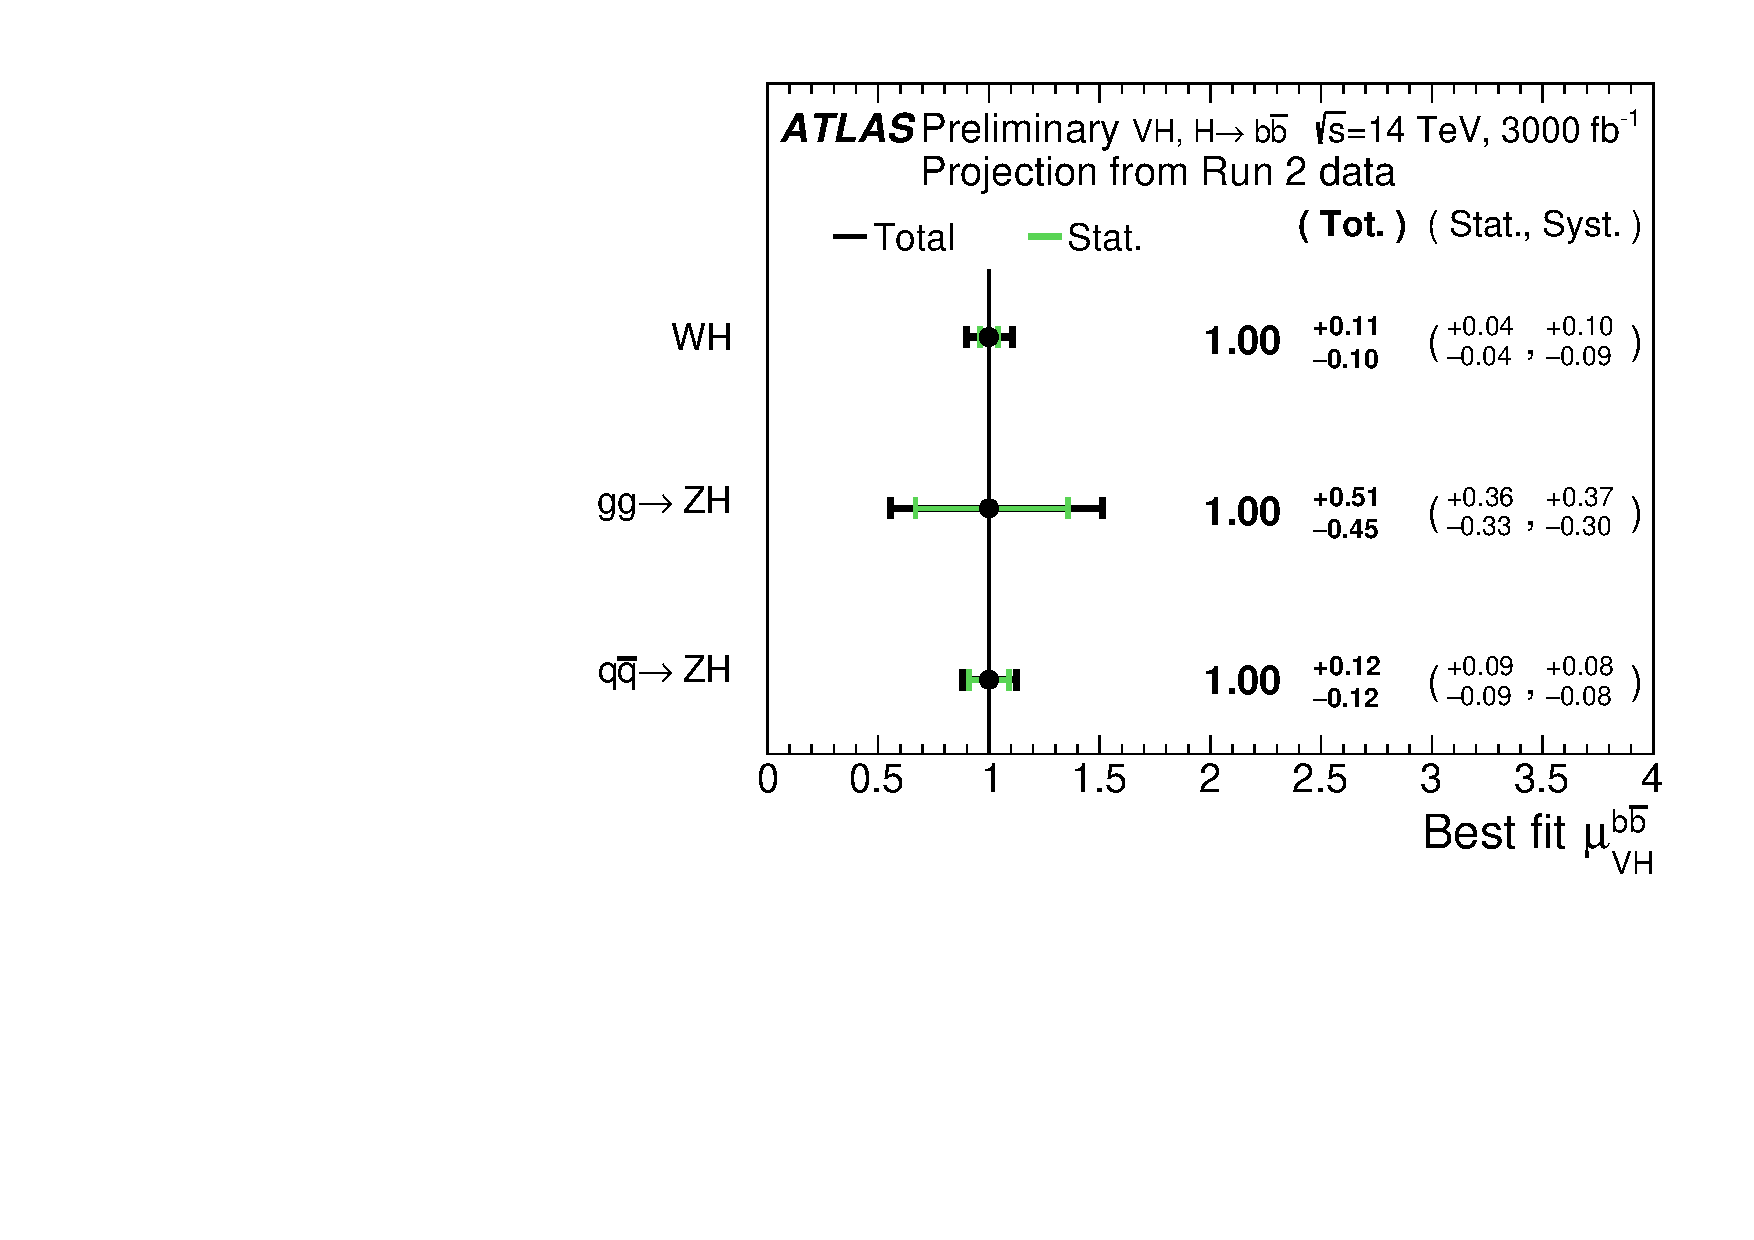
\includegraphics[width=0.45\textwidth]{hbbATLAS.png}
\end{center}
\caption{Extrapolation of the uncertainties estimated by the CMS collaboration (left) and by the ATLAS collaboration (right). The figure gives the uncertainties per-channel and on the combined signal strengths on the left, and per-production mode on the right. Values are given for the S1 (with Run~2 systematic uncertainties~\cite{HIG16044}) and S2 (with YR18 systematic uncertainties) scenarios, as well as a scenario in which all systematic uncertainties are removed. Only the S2 scenario is presented in the plot by the ATLAS collaboration (S1 is presented in Table \ref{tab:vhbb_uncertbreakdown}).}
\label{fig:vhbb_proj_bars}
\end{figure}
\begin{table}[th!]
\begin{center}
{
\caption{Contributions of particular groups of uncertainties, expressed as percentages, in S1 (with Run~2 systematic uncertainties~\cite{HIG16044}) and S2 (with YR18 systematic uncertainties) for the CMS and ATLAS analysis. The total uncertainty is decomposed into four components: signal theory, background theory, experimental and statistical. In the CMS results, the signal theory uncertainty is further split into inclusive and acceptance parts, and the contributions of the b-tagging and JES/JER uncertainties to the experimental component are also given. In the ATLAS results, the contributions of the four groups of uncertainties are presented for $pp\to WH$, $qq\to ZH$ and $gg\to ZH$ separately.}
\label{tab:vhbb_uncertbreakdown}
\begin{tabular}{l | c c | c c c c c c }
\hline\hline
Experiment & \multicolumn{2}{c |}{CMS} &  \multicolumn{6}{c}{ATLAS}\\
Process & \multicolumn{2}{c |}{$pp\to VH$} & \multicolumn{2}{c}{$pp\to WH$}& \multicolumn{2}{c}{$qq\to ZH$}& \multicolumn{2}{c}{$gg\to ZH$}\\ 
\hline
Scenario & S1 & S2 &  S1 & S2  & S1 & S2 & S1 & S2 \\
Total uncertainty   & 7.3\%  & 5.1\% & xx\% & xx\% &xx\% & xx\% & xx\% & xx\% \\
\hline
Statistical uncert. & 3.2\% & 3.2\% & xx\% & xx\% & xx\% & xx\% & xx\% & xx\% \\
Experimental uncert. & 2.6\% & 2.2\% & xx\% & xx\% & xx\% & xx\% & xx\% & xx\% \\
\quad b-tagging & 2.2\%  & 2.0\% & -- & -- & --& -- & -- & -- \\
\quad JES and JER & 0.7\%  & 0.6\% & -- & -- & --& -- & -- & -- \\
Signal theory uncer.& 5.4\% & 2.6\% & xx\% & xx\% & xx\% & xx\% & xx\% & xx\% \\
\quad Inclusive & 4.6\% &2.2\% & -- & -- & -- & -- & -- & -- \\
\quad Acceptance & 2.7\% &1.3\%& -- & -- & --& -- & -- & --\\
Background uncert. & 2.8\% & 2.3\% & xx\% & xx\% & xx\% & xx\% & xx\% & xx\% \\
\hline\hline
\end{tabular}
} % end footnotesize
\end{center}
\end{table}

Both in scenario S1 and S2 the largest component of the systematic uncertainty is theoretical. This arises from the uncertainty in the gluon-induced $ZH$ ($gg\to ZH$) production cross section due to QCD scale variations. The $gg\to ZH$ process contributes a small fraction of the total $ZH$ process. Despite this, the uncertainty in the production cross section for this process due to QCD scale variations  becomes dominant because it is very large: 25\% for the $gg\to ZH$ process, compared to approximately 0.7\% for the $qq\to ZH$ process \cite{deFlorian:2016spz}. The theoretical uncertainties on the $gg\to ZH$ production are reduced to 15\% in the S2.
An important contribution to the uncertainties are due to category-acceptance uncertainties in the dominant $Z+bb$ and $W+bb$ backgrounds due to QCD scale variations, as well as the uncertainty in the $qq\to ZH$ and $WH$ production
cross section due to QCD scale variations. In extrapolation to the scenario S2 done by the CMS Collaboration, these four most important uncertainties contribute 1.6\%, 1.5\%, 1.3\% and 1.2\% (absolute) to
the total uncertainty of 5.1\%, respectively. To improve the precision of the measurement it is therefore important to improve these theoretical uncertainties.


In the future, and at the HL-LHC in particular, the b-tagging efficiency may change. The conditions could worsen the efficiency, but
at the same time new detectors and new techniques could also lead to an improvement in the b-tagging efficiency. 
The effect of changes in b-tagging efficiency on the overall signal strength uncertainty has been evaluated by the CMS collaboration. 
Figure \ref{fig:vhbb_btageff} shows the results of the projection  assuming various reductions and improvements in the b-tagging efficiency relative to the performance of the b-tagging algorithm used in the analysis.
A 10\% improvement in the b-tagging efficiency leads to a relative improvement in the signal strength uncertainty of up to 6\%.

\begin{figure}[h!]
\begin{center}
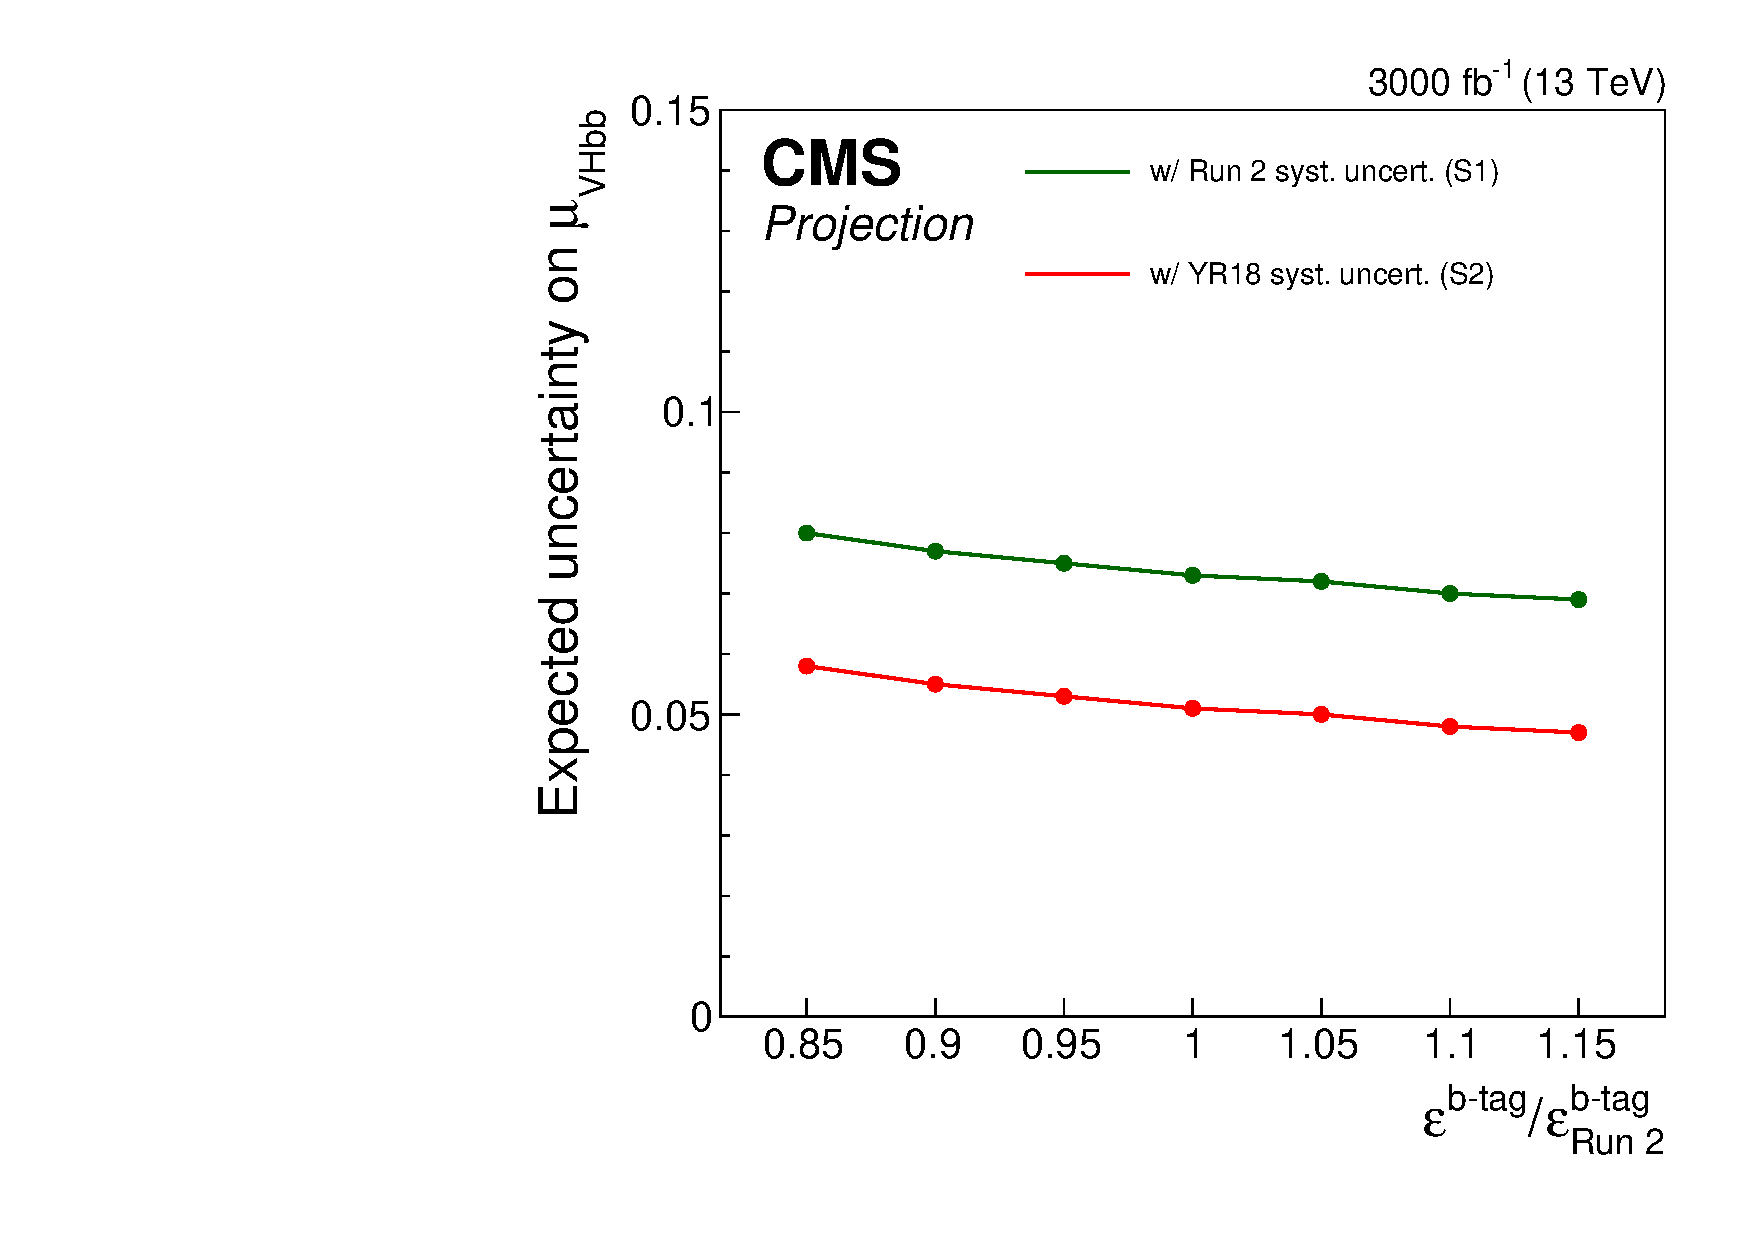
\includegraphics[width=0.5\textwidth]{\main/section2/plots/channels/BTagEff_Fig_3abonly.pdf}
\end{center}
\caption{Effect of varying the b-tagging efficiency ($\varepsilon^{\text{b-tag}}$) on the uncertainty in the signal strength measurement when considering all systematic uncertainties.}
\label{fig:vhbb_btageff}
\end{figure}


\subsubsection{$H \to \mu^{+}\mu^{-}$}
%\begin{center}
%{\it Written by: P. Francavilla}
%\end{center}
The  $H \to \mu^{+}\mu^{-}$ analyses search for a narrow peak in the dimuon invariant mass over a smooth background which is dominated by the irreducible $Z\to\mu^{+}\mu^{-}$ background. Events must have two opposite-charge muons passing loose quality selections to retain as much signal as possible. 
The overall sensitivity to this decay mode is improved by categorizing the selected events into two set of signal regions which separate the signal events produced in vector boson fusion  (catheterized by the presence of jets) from the rest (produced in gluon fusion). These two set of signal regions are further divided in sub-categories based on multivariate classifiers, or based on signal purity and muon momemtum resolution. More details on the analysis methods can be found in the most recent searches of the  $H \to \mu^{+}\mu^{-}$ channels published by ATLAS \cite{Aaboud:2017ojs} and CMS \cite{HIG-17-019}.  

The studies presented here are performed based on a previous analysis, in which the ATLAS Collaboration analyzed the 2015-2017 proton-proton collision dataset collected at $\sqrt{s} = 13\,\UTeV$, which corresponds to an integrated luminosity of 79.8\fbinv \cite{Aaboud:2017ojs}. 
In addition to the standard extrapolation procedure, the di-muon signal widths are reduced  by 15-30\% thanks the improvements expected from the performance of the tracker system upgrade ITk\cite{Collaboration:2285585}.
In this analysis, the $Z\to\mu^{+}\mu^{-}$ background is fully determined by data, and it is modelled by fitting the di-muon invariant mass $m_{\mu\mu}$ distribution in each category using a Breit-Wigner function convolved with a gaussian summed to a smooth function.

The results of the Run-2 analysis with 79.8 fb$^{-1}$ of data at $\sqrt{s} = 13\,\UTeV$ are compared to the results of 
HL-LHC with 3000\fbinv of data at s $\sqrt{s} = 14\,\UTeV$ in Table \ref{tab:hmumu_proj}.
 \begin{table}[th!]
\begin{center}
{
\caption{Expected precisions on the signal strength measurement in the $H\to\mu^{+}\mu^{-}$ channels with 3000\fbinv of HL-LHC data with the two systematic uncertainties scenarios. For the HL-LHC extrapolation, the improved ITk resolution has been emulated. }
\label{tab:hmumu_proj}
\begin{tabular}{l | c c}
\hline\hline\\
Experiment, Process & \multicolumn{2}{c}{ATLAS, Combination}\\ 
\hline\\
Scenario  & S1 & S2  \\
%Luminosity & 79.8 \fbinv&\multicolumn{2}{c}{3000 \fbinv}\\
Total uncertainty   & xx\%  & xx\% \\
\hline
Statistical uncert. & xx\% & xx\% \\
Experimental uncert. & xx\% & xx\% \\
Theory uncer.& xx\% & xx\% \\
\hline\hline
\end{tabular}
} % end footnotesize
\end{center}
\end{table}
In both the S1 and S2 scenarios, the analysis is limited by the statistical uncertainty, while the leading systematic uncertainty are the bias introduced by the choice of the function describing the background (spurious signal uncertainty), and the uncertainties on the modelling of the signal (their reduction in S2 contributes to an overall improvement of 10\% on the precision of the measurement).


\begin{comment}
\subsubsection{$H \to bb$}
{\it To be written by: P. Francavilla, A. de Wit}

\wip{Text currently reflects CMS studies only. Should be updated to reflect ATLAS and CMS studies.
Differences for ATLAS: 
-> the analysis is the observation (78.9 fb-1)
-> tagger is named MVa, and we use a 70\% WP
-> mbb is improved with muon in jet correction and ptReco, + kinematic fit for 2 leptons
-> add the mu for ATLAS
-> Add the results from ATLAS
}

%dataset of the extrapolation
The ATLAS and CMS Collaborations have both reported the observation of the $\text{H}\to\text{bb}$ decay \cite{Aaboud:2018zhk,Sirunyan:2018kst}.
The studies presented here are performed by extrapolating the most recent ATLAS $\text{H}\to\text{bb}$ measurements using a dataset corresponding to an integrated luminosity of 78.9 \fbinv, and by extrapolating a previous analysis by the CMS Collaboration. In this previous analysis evidence for the $\text{H}\to\text{bb}$ decay in the $\text{VH}$ production mode was reported using a dataset corresponding to an integrated luminosity of 35.9\fbinv \cite{HIG16044}. 

%channels
The analyses make use of leptonic decays of the vector boson which is produced in association with the Higgs boson. The final states
of the $\vh$ system covered in the analyses always contain two b-jets and either zero, one or two electrons or muons. Both leptons are required to have the same flavour in the two lepton selection.
%backgrounds
Major backgrounds arising from SM production of vector boson plus heavy- or light-flavour jets, in addition to \ttbar production, are 
controlled and constrained via dedicated control regions. Multivariate energy regression techniques are used to improve the b-jet energy resolution, and a boosted decision tree is used to improve the discrimination 
between signal and background. The distribution of this multivariate discriminator is used as the discriminating
variable in the signal extraction fit. 
%results
The signal strength observed in the CMS analysis is 
$\mu_{\text{VHbb}} = 1.19^{+0.21}_{-0.20}\text{ (stat) }^{+0.34}_{-0.32}\text{ (syst) }$. The projected uncertainties on the signal strength reported here assume $\mu_{\text{vHbb}} = 1$.

Figure \ref{fig:vhbb_proj_bars} shows the per-channel signal strength uncertainty as well as the uncertainty on the overall signal strength, showing results for all three scenarios described above. These results are for the projection of the CMS analysis.
The large improvement in the signal strength uncertainty for the 1-lepton channel, which is most sensitive to the WH production
mode, is caused by the integrated luminosity scaling of an uncertainty in the modelling of the $\PW$ boson $\pT$ distribution. This uncertainty dominates this channel
in scenario S1.

\begin{figure}[h!]
\begin{center}
% 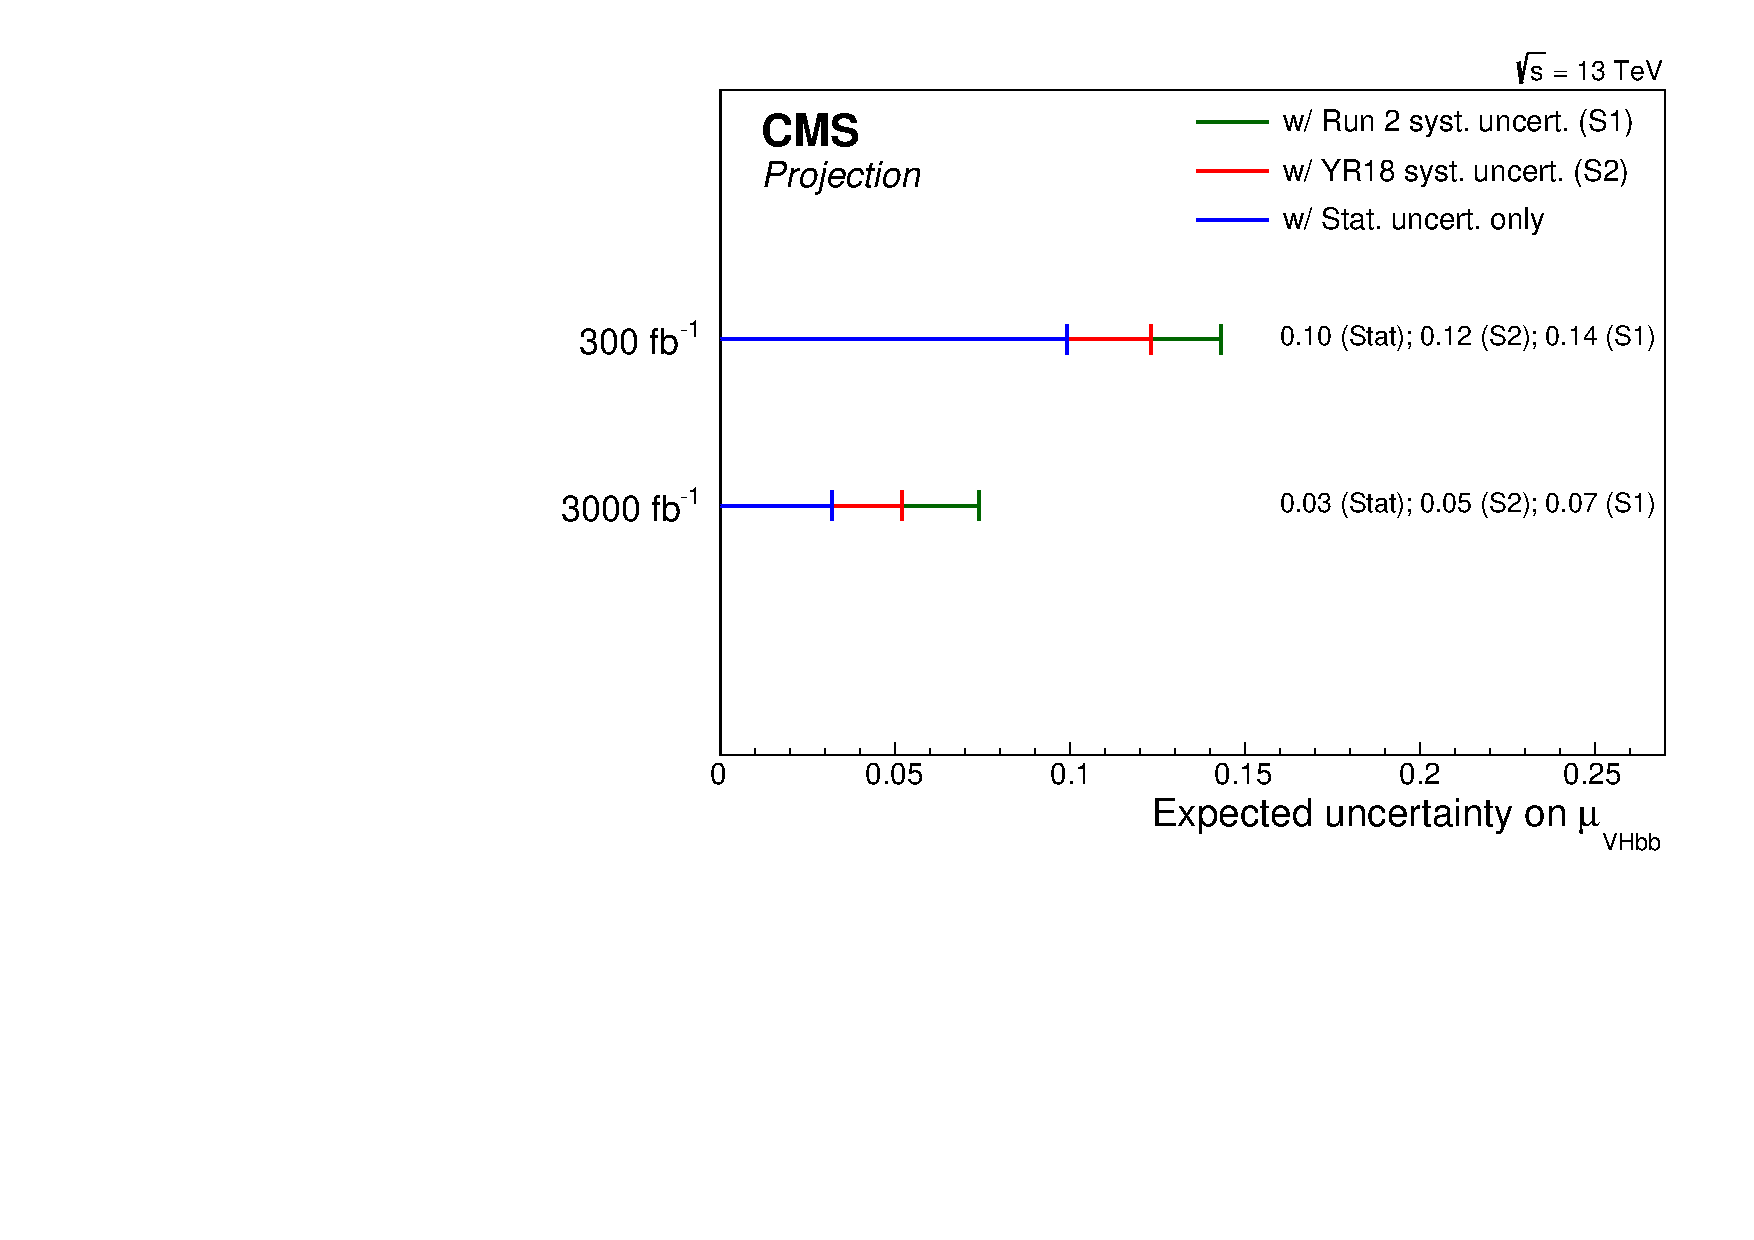
\includegraphics[width=0.48\textwidth]{\main/section2/plots/channels/Uncert300and3000.pdf}
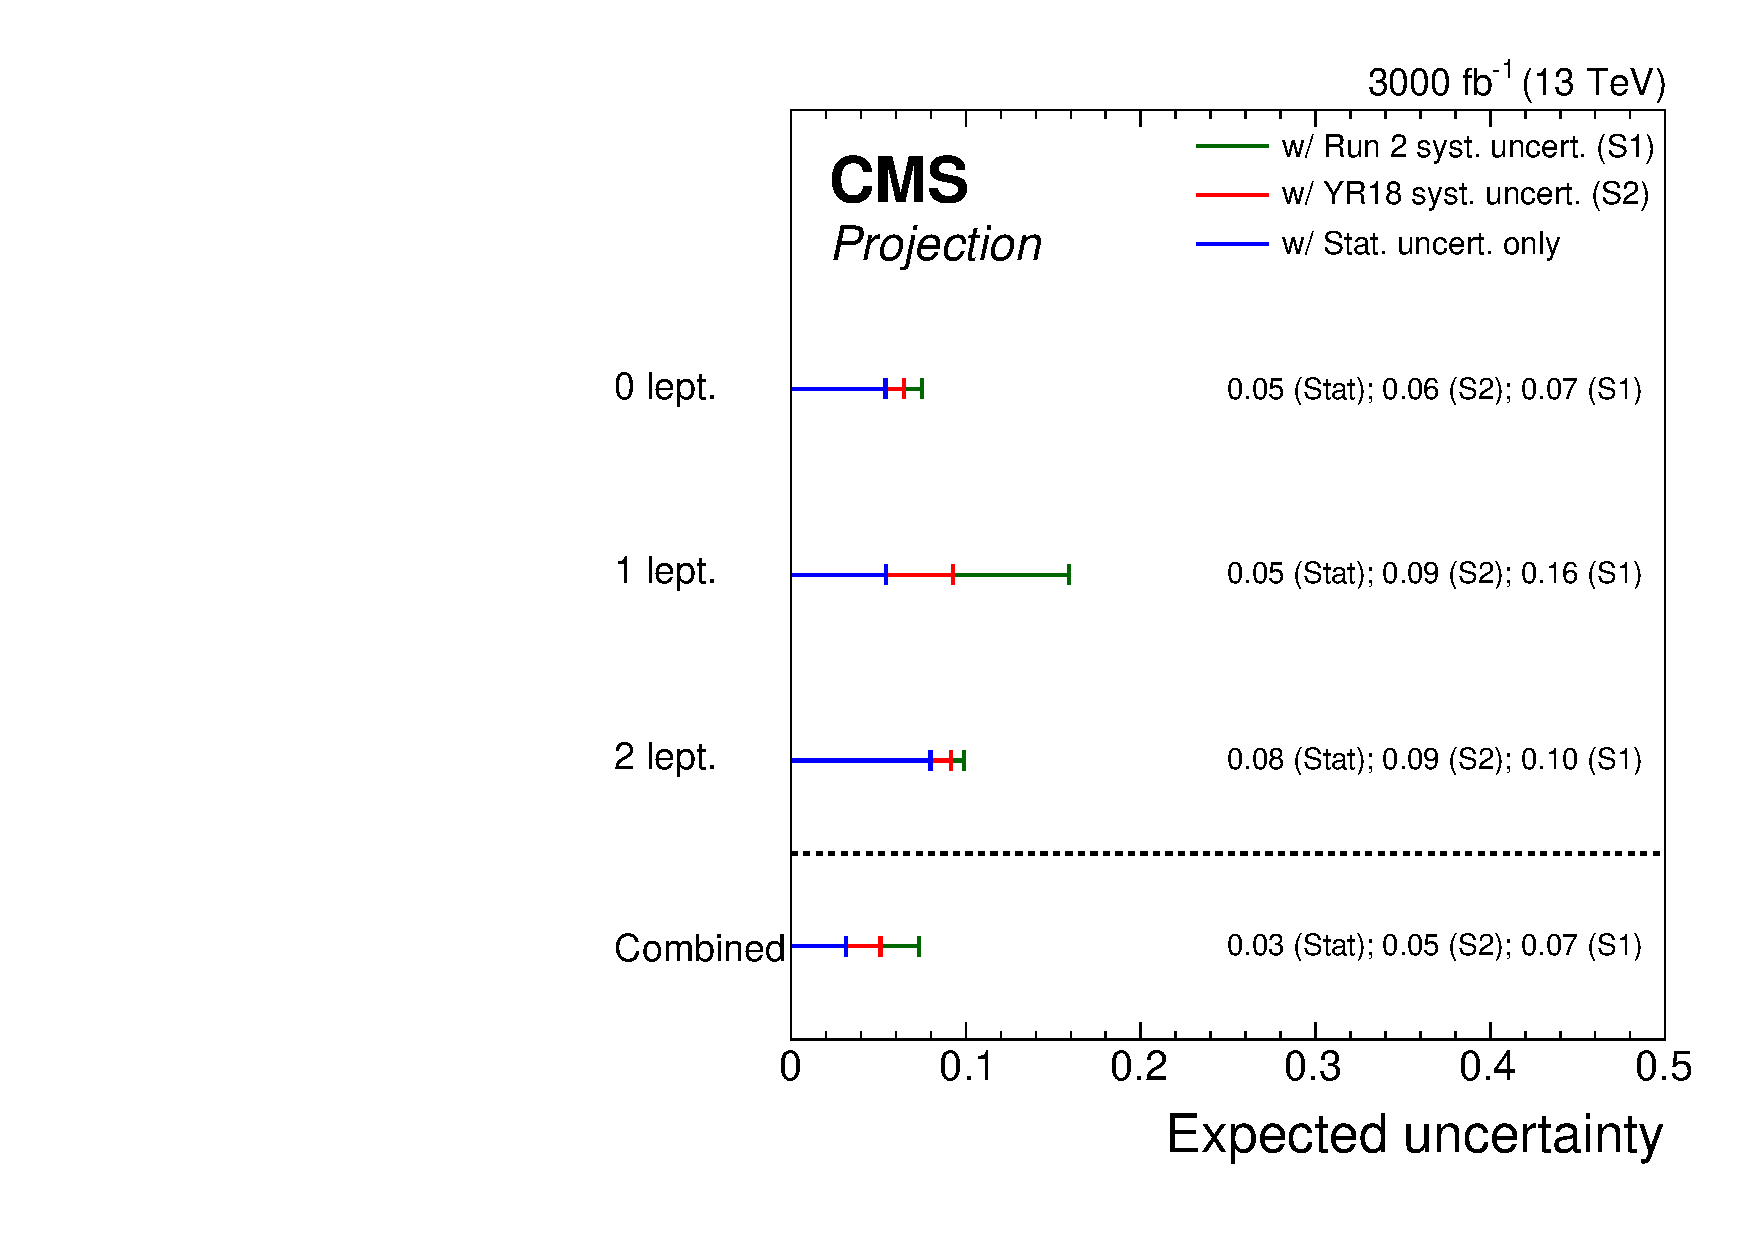
\includegraphics[width=0.6\textwidth]{\main/section2/plots/channels/ccc_3000fb_all_condensed.pdf}
\end{center}
\caption{Uncertainties in the per-channel and combined signal strengths. Values are given for the S1 (with Run~2 systematic uncertainties~\cite{HIG16044}) and S2 (with YR18 systematic uncertainties) scenarios, as well as a scenario in which all systematic uncertainties are removed.}
\label{fig:vhbb_proj_bars}
\end{figure}

The contributions of different sources of uncertainty in scenarios S1 and S2 for the projection of the CMS analysis are shown in Table~\ref{tab:vhbb_uncertbreakdown}.
Both in scenario S1 and S2 the largest component of the systematic uncertainty is theoretical. This arises from the uncertainty in the gluon-induced $\zh$ ($\ggZH$) production cross section due to QCD scale variations. The $\ggZH$ process contributes a small fraction of the total $\zh$ process. Despite this, the uncertainty in the production cross section for this process due to QCD scale variations 
becomes dominant because it is very large: 25\% for the ggZH process, compared to approximately 4\% for the ZH process \cite{deFlorian:2016spz}.
The next most important uncertainties are category-acceptance uncertainties in the dominant Z+bb and W+bb backgrounds due to QCD scale variations, as well as the uncertainty in the ZH and WH production
cross section due to QCD scale variations. In scenario S2 these four most important uncertainties contribute 1.6\%, 1.5\%, 1.3\% and 1.2\% (absolute) to
the total uncertainty of 5.1\%, respectively. To improve the precision of the measurement it is therefore important to improve these theoretical uncertainties.

\begin{table}[th!]
\begin{center}
{
\caption{Contributions of particular groups of uncertainties, expressed as percentages, in S1 (with Run~2 systematic uncertainties~\cite{HIG16044}) and S2 (with YR18 systematic uncertainties) for the CMS analysis. The total uncertainty is decomposed into four components: signal theory, background theory, experimental and statistical. The signal theory uncertainty is further split into inclusive and acceptance parts, and the contributions of the b-tagging and JES/JER uncertainties to the experimental component are also given.}
\label{tab:vhbb_uncertbreakdown}
\begin{tabular}{l c c}
 & S1 & S2\\
Total uncertainty   & 7.3\%  & 5.1\% \\
\hline
Signal theory uncertainty& 5.4\% & 2.6\%\\
\quad Inclusive & 4.6\% &2.2\%\\
\quad Acceptance & 2.7\% &1.3\%\\
Background theory uncertainty & 2.8\% & 2.3\%\\
Experimental uncertainty & 2.6\% & 2.2\% \\
\quad b-tagging & 2.2\%  & 2.0\% \\
\quad JES and JER & 0.7\%  & 0.6\% \\
Statistical uncertainty & 3.2\% & 3.2\%\\
\end{tabular}
} % end footnotesize
\end{center}
\end{table}

In the future, and at the HL-LHC in particular, the b-tagging efficiency may change. The conditions could worsen the efficiency, but
at the same time new detectors and new techniques could also lead to an improvement in the b-tagging efficiency. 
The effect of changes in b-tagging efficiency on the overall signal strength uncertainty is evaluated. Changes in the b-tagging
efficiency are emulated by scaling the rates of processes with a single b-tag by the change in b-tagging efficiency, and scaling the 
rates of processes with two b-tags by the change in b-tagging efficiency squared. The modifications are applied only to the efficiency to select genuine b-jets; the mistagging rates for light quark and gluon jets remain unchanged.

Figure \ref{fig:vhbb_btageff} shows the results of the projection of the CMS analysis assuming various reductions and improvements in the b-tagging efficiency relative to the performance of the b-tagging algorithm used in the analysis.
A 10\% improvement in the b-tagging efficiency leads to a relative improvement in the signal strength uncertainty of up to 6\%. The improvements on the signal strength precision are limited because the uncertainty is dominated by theoretical sources. When neglecting inclusive signal theory uncertainties this improvement becomes up to 8\%.


\begin{figure}[h!]
\begin{center}
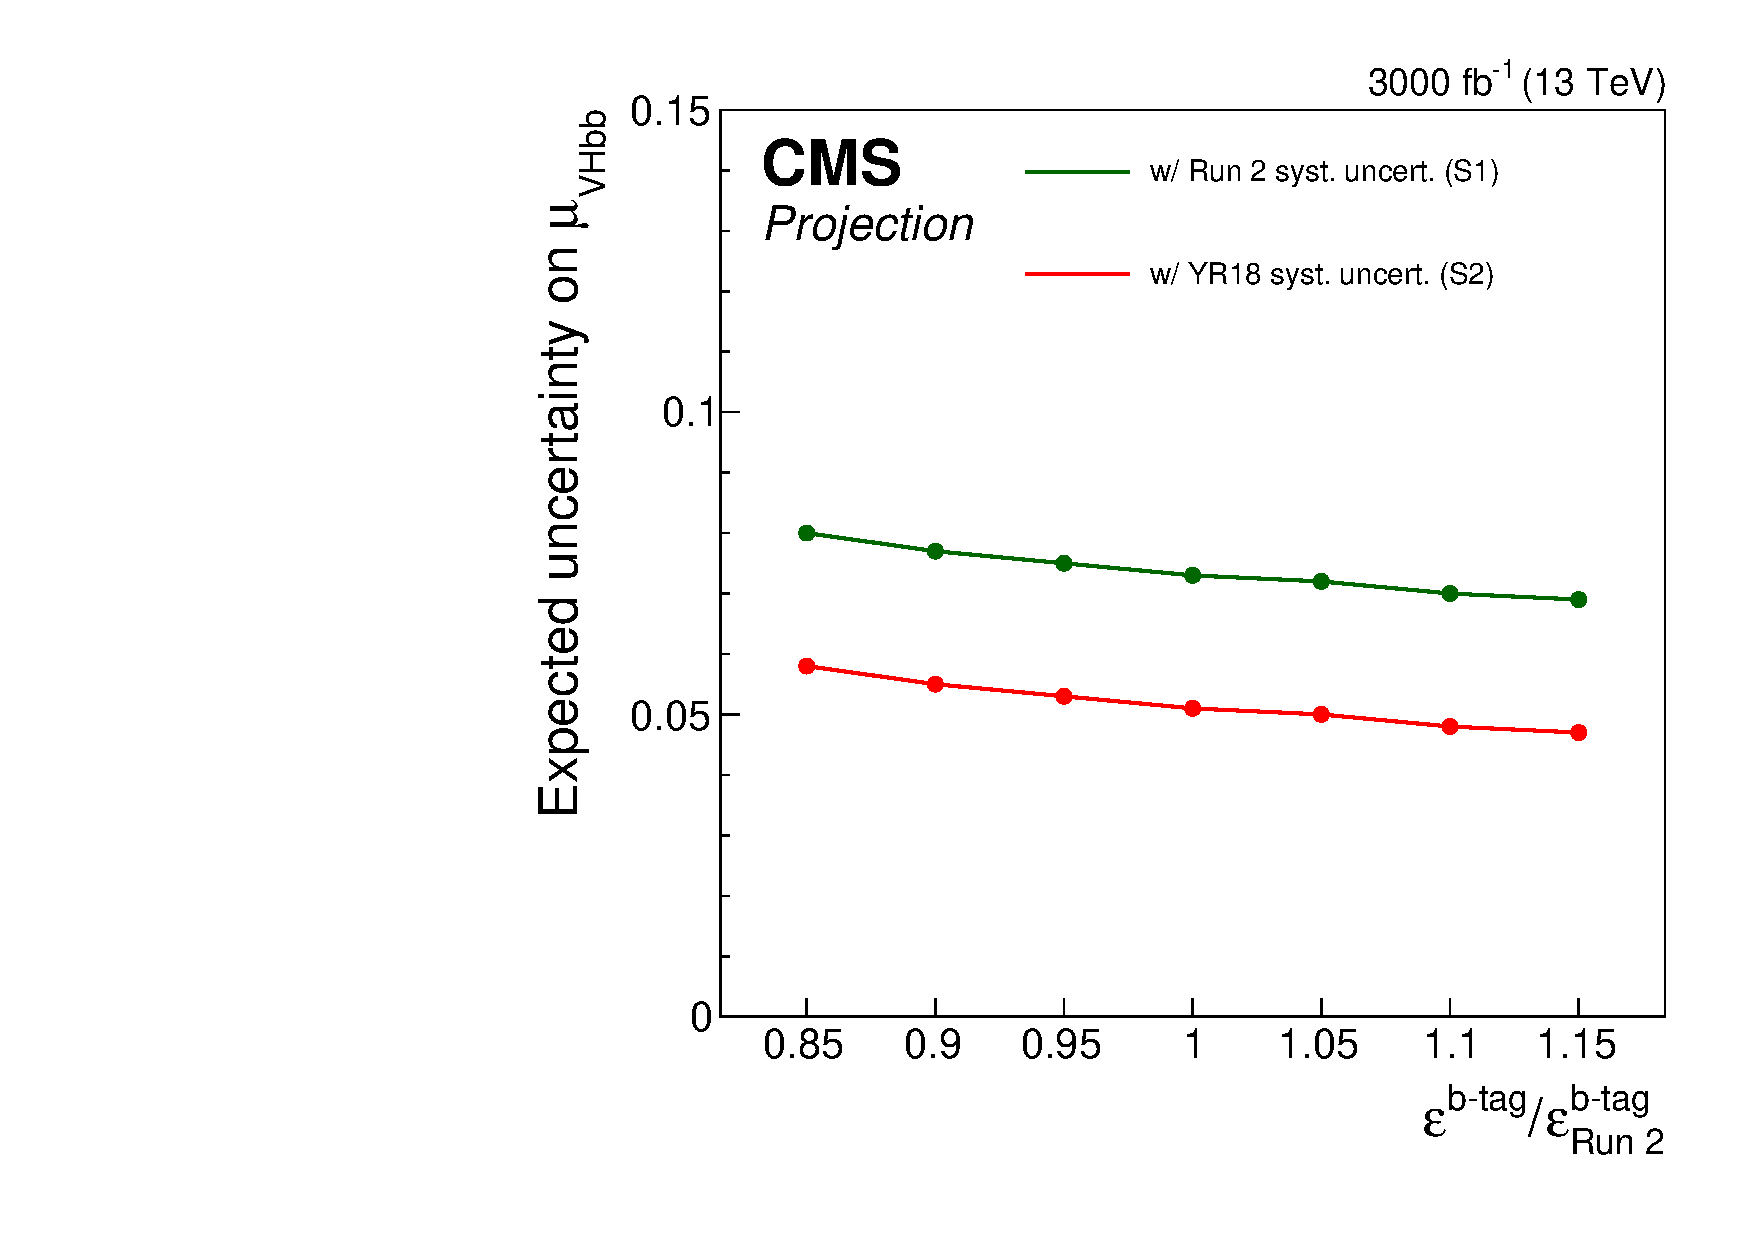
\includegraphics[width=0.5\textwidth]{\main/section2/plots/channels/BTagEff_Fig_3abonly.pdf}
\end{center}
\caption{Effect of varying the b-tagging efficiency ($\varepsilon^{\text{b-tag}}$) on the uncertainty in the signal strength measurement when considering all systematic uncertainties.}
\label{fig:vhbb_btageff}
\end{figure}

\end{comment}